
\chapter{La couche physique et la couche logique}

Nous venons de voir comment coder des informations en binaire. Nous allons ici nous intéresser à la manière de manipuler ces représentations et notamment proposer des algorithmes permettant d'effectuer des opérations arithmétiques sur les représentations binaires des nombres. Pour le moment, on ne sait faire ces opérations que sur le papier mais, pour automatiser des calculs, il faut mettre au point des mécanismes physiques (mécaniques, électroniques, optiques) réalisant ces opérations. On commencera par introduire le transistor qui est l'élément majeur des circuits électroniques que nous allons présenter\footnote{Un microprocesseur des années 1970 comptait quelques milliers de transistor. En 2015, les microprocesseurs multi-coeurs contiennent une dizaine de milliards de transistors ($10.10^{9}$). Source : \protect\url{https://en.wikipedia.org/wiki/Transistor_count}} et très vite, nous en ferons l'abstraction en introduisant les portes logiques à partir desquelles nous élaborerons différents circuits particuliers qui nous permettrons de construire notre première architecture.

\section{Un peu d'électronique}

Avant de voir plus en détails comment se construit un ordinateur, il faut introduire quelques éléments d'électronique pour comprendre comment représenter physiquement un bit ainsi que des circuits électroniques permettant de manipuler ces signaux. Ces circuits vont principalement reposer sur le transistor et nous allons voir pourquoi ce composant est particulièrement bien adapté. 

%Attention, les circuits électroniques présentés dans les sections suivantes sont à considérer comme des \textbf{circuits de principe}. Bien qu'il soient valables, ils ne sont pas utilisés en pratique pour réaliser les fonctions qu'on va présenter pour diverses raisons de performances. Je vous suggère de vous diriger vers un véritable cours d'électronique pour en savoir plus à ce sujet.

\subsection{Niveaux logiques et valeurs de tension}

La représentation d'un bit se fait en électronique par des niveaux de tension. Disons\footnote{Les circuits logiques utilisent généralement des tensions entre 0V et 3.3V ou entre 0V et 5V. On utilise ici 1V à titre d'illustration.}, par exemple, $0$V pour un bit au niveau bas $b=0$ et $1$V pour un bit au niveau haut $b=1$. Cela étant dit, quel est l'état binaire d'une tension à $0.75$ V? probablement $b=1$; $0.25$ V ? probablement $b=0$ et qu'en est-il de $0.49$V et $0.51$V ? A cause des défauts de fabrication, des perturbations possibles de l'environnement du circuit, il est nécessaire d'introduire des tolérances et de définir des domaines de tension acceptable pour définir chacun des niveaux logiques. Les circuits électroniques que nous allons considérer vont transformer des tensions d'entrées $V_{in}$ en des tensions de sortie $V_{out}$ (fig. \ref{fig:VTC}a) et la fonction reliant les deux est appelée \textbf{fonction caractéristique de transfert} (\emph{Voltage Transfer Characteristics}).

\begin{figure}[htbp]
\centering\begin{tabular}{cc}
\includegraphics[width=0.5\linewidth]{Figs/vtc.pdf}& 
\includegraphics[width=0.5\linewidth]{Figs/VTC_connect.pdf}\\
a) & b)
\end{tabular}
\caption{\label{fig:VTC} a) Vision schématique d'un circuit transformant une tension $V_{in}$ en une tension $V_{out}$. La fonction reliant les deux est la fonction caractéristique de transfert. b) Des marges de bruit doivent être introduites pour garantir le bon fonctionnement de composants interconnectés. }
\end{figure}

Les fabricants définissent des domaines pour les entrées et sorties dans lesquels ils garantissent le fonctionnement de leur circuit :
\begin{itemize}
\item pour les entrées :
\begin{itemize}
\item $v_{il}$ : tension maximale d'entrée pour que le composant la considère à l'état bas $b_{in} = 0$
\item $v_{ih}$ : tension minimale d'entrée pour que le composant la considère à l'état haut $b_{in} = 1$
\end{itemize}
\item pour les sorties :
\begin{itemize}
\item $v_{ol}$ : tension maximale de sortie que le composant produit pour une sortie à l'état bas $b_{out} = 0$
\item $v_{oh}$ : tension minimale de sortie que le composant produit pour une sortie à l'état haut $b_{out} = 1$
\end{itemize}
\end{itemize}

%\todo{Quelques exemples de valeur vil, vol, ... à partir des liens en commentaire dans le latex}.\\


Quelle que soit la fonction réalisée par le circuit, le fabricant garantie que si l'entrée représente un état binaire valide ($V_{in} \in [0, v_{il}] \cup [v_{ih}, V_{cc}]$), alors la sortie représentera un état binaire valide ($V_{out} \in [0, v_{ol}] \cup [v_{oh}, V_{cc}]$). Par ailleurs, pour prendre en compte les imperfections de son circuit, les tolérances de sortie sont plus strictes que les tolérances d'entrée : une sortie est considérée à l'état haut si $v_{out} \geq v_{oh} > v_{ih}$ et à l'état bas si $v_{out} \leq v_{ol} < v_{il}$. En effet, considérons que nous interconnections deux composants comme sur la figure~\ref{fig:VTC}b. Différentes sources de bruit dûes à l'environnement du circuit conduisent au fait que le potentiel de sortie $V_{oA}$ est différent du potentiel d'entrée $V_{iB}$. Le potentiel de sortie $V_{oA}$ ne doit pas être vu comme un potentiel constant mais comment étant perturbé par un certain bruit. Si on définit $v_{ol} = v_{il}$, et que $V_{oA} = v_{ol}$, i.e. la tension maximale pour indiquer un niveau logique bas en sortie de A, la perturbation peut conduire à ce que ce niveau bas soit considéré comme invalide pour le composant B. C'est donc pour garantir qu'une sortie valide demeure une entrée valide, malgré le bruit de transimission, qu'on impose à ce que $v_{ol} < v_{il}$ et $v_{oh} > v_{ih}$. Les différences $v_{il} - v_{ol}$ et $v_{oh} - v_{ih}$ sont appelées \emph{marges de bruit}. Il y aurait beaucoup d'autres choses à dire sur la compatibilité des circuits interconnectés mais nous nous arrêterons là dans ce cours et je vous renvois vers un cours d'électronique pour en savoir plus. 

%\begin{figure}[htbp]
%\centering\includegraphics[width=0.5\linewidth]{Figs/VTC_connect.pdf}
%\caption{\label{fig:VTC_connect} Des marges de bruit doivent être introduites pour garantir le bon fonctionnement de composants interconnectés.}
%\end{figure}

\begin{figure}[htbp]
\centering\includegraphics[width=0.5\linewidth]{Figs/vtc_forbidden_labels.pdf}\includegraphics[width=0.5\linewidth]{Figs/vtc_forbidden.pdf}
\caption{\label{fig:VTC_forbidden} Les domaines interdits pour la fonction caractéristique de transfert sont représentés en rouge. Quelle que soit la fonction réalisée par le circuit, la fonction caractéristique de transfert devra toujours éviter les domaines interdits pour s'assurer qu'une entrée valide donne toujours une sortie valide. La fonction représentée en noir est une fonction valide.}
\end{figure}

Pour en revenir à un seul composant, notez que rien n'interdit de produire une sortie valide si l'entrée est invalide. Cela conduit ainsi à définir des domaines interdits pour la fonction caractéristique de transfert comme illustré sur la figure \ref{fig:VTC_forbidden}, domaines dans lesquels il est interdit de faire passer la fonction de transfert caractéristique.

Raisonner avec la fonction caractéristique de transfert permet d'identifier une caractéristique des circuits permettant de manipuler des ``représentations binaires'' : ce circuit doit utiliser des composants non linéaires. Au début de l'informatique, dans les années 1930-1940, on utilisait des relais électromécaniques comme par exemple le relais de Joseph Henry illustré sur la figure~\ref{fig:relay}.

\begin{figure}[htbp]
\centering\includegraphics[width=0.5\linewidth]{eps/relay.jpg}
\caption{\label{fig:relay} Relai électromécanique de Joseph Henry. Branchons $v_{out}$ sur la patte 1, $v_{cc}$ sur la patte 4, la masse sur la patte 5 et $v_{in}$ sur la bobine, on obtient alors un inverseur. Si $v_{in}=0$, la languette métallique 10 relie la patte 1 à la patte 4 donc $v_{out}=v_{cc}$. Si $v_{in} = v_{cc}$, le champ magnétique de la bobine conduit à placer la languette métallique 10 en contact avec la pièce 12 et donc $v_{out}=0$. Illustration de \url{http://history-computer.com}.}
\end{figure}

En pratique, les relais sont encombrants, sujets aux interférences, peu robustes dans le temps puisque mécaniques, gourmands en énergie, ... Dans les années 1950 est apparu le transistor, un interrupteur électronique commandable qui a révolutionné l'informatique.

\subsection{Transistors CMOS et inverseur}

Comme nous venons de le voir, il nous faut disposer d'un composant électronique dont la fonction caractéristique de transfert est non linéaire. Le transistor, apparu dans les années 1950 est justement un composant non linéaire. Il existe plusieurs technologies pour réaliser des transistors (TTL, MOS, ..) et ce n'est pas le sujet de ce cours que de les présenter. On ne s'intéressera qu'à une technologie : le transistor MOSFET (Metal Oxyde Field Effect Transistor) et on va s'abstraire du transistor en le voyant comme un interrupteur commandable. Des transistors TTL et MOS sont représentés sur la figure \ref{fig:transistor_bipolaire} et les transistors MOS sont ceux représentés sur les figures \ref{fig:transistor_bipolaire}c, d. Je vous renvois vers un cours de physique des semi-conducteurs pour comprendre le fonctionnement de ces transistors. Nous retiendrons ici deux états de fonctionnement du transitor (passant/saturé ou bloqué) et que l'état dans lequel se trouve le transistor dépends de la différence de potentiel entre la grille et la source.

\begin{figure}
\begin{center}
\begin{tabular}{cccc}
\begin{circuitikz}
\draw	(0,0) node[npn](npn1){};
\node at ($(npn1.B) - (0.5,0)$) {Base};
\node at ($(npn1.E) - (0, 0.5)$) {Emetteur};
\node at ($(npn1.C) + (0, 0.5)$) {Collecteur};
\end{circuitikz} &
\begin{circuitikz}
\draw	(0,0) node[pnp](pnp1){};
\node at ($(pnp1.B) - (0.5,0)$) {Base};
\node at ($(pnp1.E) + (0, 0.5)$) {Emetteur};
\node at ($(pnp1.C) - (0, 0.5)$) {Collecteur};
\end{circuitikz} &
\begin{circuitikz}
\draw (0, 0) node[nmos] (nmos1) {};
\node at ($(nmos1.gate) - (0.5,0)$) {Grille};
\node at ($(nmos1.drain) + (0, 0.5)$) {Drain};
\node at ($(nmos1.source) - (0, 0.5)$) {Source};
\end{circuitikz} &
\begin{circuitikz}
\draw (0, 0) node[pmos] (pmos1) {};
\node at ($(pmos1.gate) - (0.5,0)$) {Grille};
\node at ($(pmos1.drain) - (0, 0.5)$) {Drain};
\node at ($(pmos1.source) + (0, 0.5)$) {Source};
\end{circuitikz} \\
a) & b) & c) & d)
\end{tabular}
\end{center}
\caption{\label{fig:transistor_bipolaire} a) Transistor bipolaire NPN. b) Transistor bipilaire PNP. c) Transistor unipolaire NMOS. d) Transistor unipolaire PMOS}
\end{figure}

Pour ce qui nous concerne dans ce cours, un transistor est abstrait comme un interrupteur commandable (fig. \ref{fig:circuits_mos}a):
\begin{itemize} 
\item Pour un transistor NMOS : si \textbf{une tension nulle est appliquée à la grille}, aucun courant ne circule entre le drain et la source : \textbf{le transistor est bloqué}. Si \textbf{une tension positive est appliquée à la grille}, un courant peut circuler entre le drain et la source : \textbf{le transistor est passant}.
\item Pour un transistor PMOS : si \textbf{une tension nulle est appliquée à la grille}, un courant peut circuler entre la source et le drain : \textbf{le transistor est passant}. Si \textbf{une tension positive est appliquée à la grille}, aucun courant ne circule entre la source et le drain : \textbf{le transistor est bloqué}.
\end{itemize}
La technologie CMOS (Complementary Metal Oxyde Semi Conductor) utilise des transistors en paire PMOS et NMOS placés de manière symétrique (fig. \ref{fig:circuits_mos}b) :
\begin{itemize}
\item les PMOS sont disposés entre l'alimentation $V_{cc}$ et la sortie du circuit; on parle de réseau ``pull-up''
\item les NMOS sont disposés entre la sortie et la masse; on parle de réseau ``pull-down''
\end{itemize}

\begin{figure}[htbp]
   \begin{minipage}[c]{.56\linewidth}
\includegraphics[width=\columnwidth]{Figs/nmospmos.pdf} \\\centering a)
   \end{minipage} \hfill
   \begin{minipage}[c]{.25\linewidth}
\includegraphics[width=\columnwidth]{Figs/circuits_mos.pdf}\\\centering b)
   \end{minipage}
\caption{\label{fig:circuits_mos} a) Les transistors NMOS et PMOS peuvent être vus comme des interrupteurs commandables dont l'état dépends de la différence de potentiel entre la source et la grille. Fixant le potentiel de la source à $V_{cc}$ pour le PMOS et à la masse pour le NMOS, le transitor est commandé par le potentiel appliqué à la grille. b) En technologie CMOS, les circuits à base de transistor MOS sont construits en utilisant des paires de transistors de type P et de type N. Les types P relient toujours l'alimentation à la sortie et les types N la sortie à la masse.}
\end{figure}

Un transistor est un système physique auquel il faut un certain temps pour passer entre les états passant et bloqué. Un transistor unipolaire CMOS mets quelques picosecondes ($10^{-12}s$) pour commuter. En pratique, le transistor se trouve dans un circuit : soit un circuit de mesure, soit interconnecté avec d'autres composants. Il faut alors prendre en compte une capacité parasite de sortie et le temps de commutation est dépendant de cette capacité et des résistances internes du transistor et qui conduisent à des temps de commutation de l'ordre de la nanoseconde.

\begin{figure}[htbp]
   \begin{minipage}[c]{.46\linewidth}
\begin{circuitikz}[scale=0.7, every node/.style={scale=0.7}]
\draw[color=black, thick]
        (0,1.0) node[nmos](nmos1){}
        (0,3.0) node[pmos](pmos1){}

        (nmos1.gate) -- (pmos1.gate) node[midway] (Vin) {}
        (nmos1.drain) -- (pmos1.drain) node[midway] (Vout){} 
        (pmos1.source) to [short,-o](0,4.5) node[right]{$V_{cc}$}
        (nmos1.source) to [short](0,0.5) node[ground]{}
        (Vout) to ($(Vout) + (1.0,0)$) node[right, short] {$V_{S}$}
        (nmos1.gate) -| (Vin) to ($(Vin) + (-1.0,0)$) node[left, short] {$V_{A}$};
\end{circuitikz}\\\centering a)
   \end{minipage} \hfill
   \begin{minipage}[c]{.46\linewidth}
\tikzstyle{branch}=[fill,shape=circle,minimum size=3pt,inner sep=0pt]
\begin{tikzpicture}[thick,scale=1.5, every node/.style={scale=1.5}]
\draw[color=black,thick]
     (0,0) node[not gate US, draw, logic gate inputs=nn] (Not1) {}
     (Not1.input) -- ($(Not1.input) - (0.5,0)$) node[left] {$A$}
     (Not1.output) -- ($(Not1.output) + (0.5, 0)$) node[right] {$S$};
\end{tikzpicture}\\\centering b)
   \end{minipage}
\caption{\label{fig:not_cmos} a) \underline{\textbf{Une}} réalisation possible d'une porte NOT en technologie CMOS avec une paire de transistors PMOS et NMOS. b) Symbole normalisé (norme Américaine) d'une porte NOT. Sur ce schéma, on ne représente pas les tensions $V_{cc}$ et la masse qui sont implicites.}
\end{figure}


\paragraph{L'inverseur : } Considérons maintenant le circuit représenté sur la figure \ref{fig:not_cmos}a. La tension appliquée à la grille est appelée $V_{A}$ et le circuit est composé d'une paire de MOS de type P et de type N comme dit précédemment. Lorsqu'un état $A = 0$ (une tension suffisamment faible) est appliqué aux grilles, le transistor PMOS (du haut) est passant tandis que le transistor NMOS (du bas) est bloqué. La sortie sera donc $V_{S} = V_{cc}$ correspondant à un niveau binaire haut $S=1$. Au contraire, si un état $A=1$ (une tension suffisamment proche de $V_{cc}$) est appliqué aux grilles, le transistor PMOS (du haut) est bloqué tandis que le transistor NMOS (du bas) est passant. La sortie sera donc $V_{S} = 0$ correspondant à un niveau binaire bas $S=0$. Ces observations sont regroupées dans la table \ref{fig:table_de_verite_not}.

\begin{table}[htbp]
\centering\begin{tabular}{cc}
\begin{tabular}{c|c}
$V_{A}$ & $V_{S}$\\
\hline
0 & $V_{cc}$ \\
$V_{cc}$ & 0
\end{tabular}&
\begin{tabular}{c|c}
$A$ & $S$ \\
\hline
0 & 1\\
1 & 0
\end{tabular}\\
a) & b)
\end{tabular}
\caption{\label{fig:table_de_verite_not} a) Tensions de sortie en fonction de la tension d'entrée pour le circuit de la figure \ref{fig:not_cmos}a. b) Traduction des niveaux de tensions en niveaux logiques sous la forme d'une \textbf{table de vérité}. Cette table de vérité corresponds au circuit appelé \textbf{inverseur}. }
\end{table}

La table de vérité \ref{fig:table_de_verite_not}b et le circuit associé de la figure \ref{fig:not_cmos}a forment ce qu'on appelle un inverseur, ici réalisé en technologie CMOS\footnote{on pourrait tout à fait réaliser un inverseur avec uniquement des PMOS ou uniquement des NMOS, ce qu'on appelle respectivement les logiques PMOS et NMOS mais pour des raisons pratiques (sensibilité aux bruits, dissipation thermique), la logique CMOS utilisant des transistors complémentaires est préférée.}. L'inverseur sera représenté sur un schéma comme sur la figure~\ref{fig:not_cmos}b.


\subsection{Portes NAND et NOR à deux entrées}
\subsubsection{Porte NAND}
Que se passe t'il si on complique un peu le circuit précédent de la porte NOT en ajoutant une autre entrée comme sur la figure \ref{fig:nand_cmos}a. En appliquant le même raisonnement que pour étudier la porte NOT, on en arrive aux tables de tensions entrées/sorties et la table de vérité \ref{fig:table_de_verite_nand}.

\begin{figure}[htbp]
   \begin{minipage}[c]{.46\linewidth}
\begin{circuitikz}[scale=0.6, every node/.style={scale=0.6}]
\draw[color=black, thick]
        (0,3.0) node[nmos](nmos1){}
        (0,5.0) node[pmos](pmos1){}
        (0,1.5) node[nmos](nmos2){}
        (2.0,5.0) node[pmos,xscale=-1](pmos2){}

        (nmos1.gate) -- ($(nmos1.gate) - (0.2,0)$) node[left] {$V_A$}
        (pmos1.gate) -- ($(pmos1.gate) - (0.2,0)$) node[left] {$V_A$}
        (nmos2.gate) -- ($(nmos2.gate) - (0.2,0)$) node[left] {$V_B$}
        (pmos2.gate) -- ($(pmos2.gate) + (0.2,0)$) node[right] {$V_B$}
        (pmos1.drain) -- (nmos1.drain)
        (pmos2.drain) -- (pmos1.drain)
        (pmos1.source) -- (pmos2.source) node[midway] (Vcc) {}
        (Vcc) to [short,-o] ($(Vcc) + (0,0.2)$) node[above] {$V_{cc}$}
        (nmos1.drain) -- ($(nmos1.drain) + (1.0, 0)$) node[right] {$V_S$}
        (nmos2.source) -- ($(nmos2.source) + (0, -0.1)$) node[ground]{};
\end{circuitikz}\\\centering a)
   \end{minipage} \hfill
   \begin{minipage}[c]{.46\linewidth}
\tikzstyle{branch}=[fill,shape=circle,minimum size=3pt,inner sep=0pt]
\begin{tikzpicture}[thick,scale=1.5, every node/.style={scale=1.5}]
\draw[color=black,thick]
     (0,0) node[nand gate US, draw, logic gate inputs=nn] (Nand1) {}
     (Nand1.input 1) -- ($(Nand1.input 1) - (0.5,0)$) node[left,above] {$A$}
     (Nand1.input 2) -- ($(Nand1.input 2) - (0.5,0)$) node[left,below] {$B$}
     (Nand1.output) -- ($(Nand1.output) + (0.5, 0)$) node[right] {$S$};
\end{tikzpicture}\\\centering b)
   \end{minipage}
\caption{\label{fig:nand_cmos} a) \underline{\textbf{Une}} réalisation possible d'une porte NAND en technologie CMOS avec deux paires de transistors PMOS et NMOS. b) Schéma abstrait d'une porte NAND. Sur ce schéma, on ne représente pas les tensions $V_{cc}$ et la masse qui sont implicites.}
\end{figure}

\begin{table}[htbp]
\centering\begin{tabular}{cc}
\begin{tabular}{cc|c}
$V_{A}$ & $V_B$ & $V_{S}$\\
\hline
0 & 0 & $V_{cc}$ \\
0 & $V_{cc}$ & $V_{cc}$ \\
$V_{cc}$ & 0 & $V_{cc}$ \\
$V_{cc}$ & $V_{cc}$ & 0
\end{tabular}&
\begin{tabular}{cc|c}
$A$ & $B$ & $S$ \\
\hline
0 & 0 & 1\\
0 & 1 & 1\\
1 & 0 & 1\\
1 & 1 & 0
\end{tabular}\\
a) & b)
\end{tabular}
\caption{\label{fig:table_de_verite_nand} a) Tensions de sortie en fonction des tensions d'entrée pour le circuit de la figure \ref{fig:nand_cmos}a. b) Traduction des niveaux de tensions en niveaux logiques sous la forme d'une \textbf{table de vérité}. Cette table de vérité corresponds au circuit appelé \textbf{NAND} (non-est) et s'écrit aussi sous forme d'équation : $S = \overline{A.B}$. }
\end{table}

NAND est la dénomination raccourcie de NOT-AND (non-et). Vous pourrez vérifier que la table de vérité obtenue peut s'écrire $S = \overline{A . B}$. Une porte NAND sera représentée dans un schéma comme sur la figure \ref{fig:nand_cmos}b.

\subsubsection{Porte NOR}

Continuons à expérimenter un peu avec les transistors CMOS et considérons maintenant le circuit de la figure \ref{fig:nor_cmos}a. En appliquant le même raisonnement que pour étudier la porte NOT, on en arrive aux tables de tensions entrées/sorties et la table de vérité \ref{fig:table_de_verite_nor}.

\begin{figure}[htbp]
   \begin{minipage}[c]{.46\linewidth}
\begin{circuitikz}[scale=0.6, every node/.style={scale=0.6}]
\draw[color=black, thick]
        (0.0,5.0) node[pmos](pmos2){}
        (0,3.5) node[pmos](pmos1){}
        (0,1.5) node[nmos](nmos1){}
        (2.0,1.5) node[nmos,xscale=-1](nmos2){}

        (nmos1.gate) -- ($(nmos1.gate) - (0.2,0)$) node[left] {$V_A$}
        (pmos1.gate) -- ($(pmos1.gate) - (0.2,0)$) node[left] {$V_A$}
        (nmos2.gate) -- ($(nmos2.gate) + (0.2,0)$) node[right] {$V_B$}
        (pmos2.gate) -- ($(pmos2.gate) - (0.2,0)$) node[left] {$V_B$}

        (nmos1.source) -- (nmos2.source) node[midway] (gnd) {}
        (gnd) -- ($(gnd) + (0, -0.1)$) node[ground]{}
        (pmos2.source) to [short,-o] ($(pmos2.source) + (0, 0.2)$) node[above] {$V_{cc}$}
        (nmos1.drain) -- (nmos2.drain)
        (pmos1.drain) -- (nmos1.drain) node[midway] (Vs) {}
        (pmos1.drain) -- ($(pmos1.drain) + (2.0, 0)$) node[right] {$V_S$};
\end{circuitikz}\\\centering a)
   \end{minipage} \hfill
   \begin{minipage}[c]{.46\linewidth}
\tikzstyle{branch}=[fill,shape=circle,minimum size=3pt,inner sep=0pt]
\begin{tikzpicture}[thick,scale=1.5, every node/.style={scale=1.5}]
\draw[color=black,thick]
     (0,0) node[nor gate US, draw, logic gate inputs=nn] (Nor1) {}
     (Nor1.input 1) -- ($(Nor1.input 1) - (0.5,0)$) node[left,above] {$A$}
     (Nor1.input 2) -- ($(Nor1.input 2) - (0.5,0)$) node[left,below] {$B$}
     (Nor1.output) -- ($(Nor1.output) + (0.5, 0)$) node[right] {$S$};
\end{tikzpicture}\\\centering b)
   \end{minipage}
\caption{\label{fig:nor_cmos} a) \underline{\textbf{Une}} réalisation possible d'une porte NOR en technologie CMOS avec deux paires de transistors PMOS et NMOS. b) Schéma abstrait d'une porte NOR. Sur ce schéma, on ne représente pas les tensions $V_{cc}$ et la masse qui sont implicites.}
\end{figure}

\begin{table}[htbp]
\centering\begin{tabular}{cc}
\begin{tabular}{cc|c}
$V_{A}$ & $V_B$ & $V_{S}$\\
\hline
0 & 0 & $V_{cc}$ \\
0 & $V_{cc}$ & 0 \\
$V_{cc}$ & 0 & 0 \\
$V_{cc}$ & $V_{cc}$ & 0
\end{tabular}&
\begin{tabular}{cc|c}
$A$ & $B$ & $S$ \\
\hline
0 & 0 & 1\\
0 & 1 & 0\\
1 & 0 & 0\\
1 & 1 & 0
\end{tabular}\\
a) & b)
\end{tabular}
\caption{\label{fig:table_de_verite_nor} a) Tensions de sortie en fonction des tensions d'entrée pour le circuit de la figure \ref{fig:nor_cmos}a. b) Traduction des niveaux de tensions en niveaux logiques sous la forme d'une \textbf{table de vérité}. Cette table de vérité corresponds au circuit appelé \textbf{NOR} (non-ou) et s'écrit aussi sous forme d'équation : $S = \overline{A+B}$. }
\end{table}

NOR est la dénomination raccourcie de NOT-OR (non-ou). Vous pourrez vérifier que la table de vérité obtenue peut s'écrire $S = \overline{A + B}$. Une porte NOR sera représentée dans un schéma comme sur la figure \ref{fig:nor_cmos}b.

\subsubsection{Et la porte AND ?}
Les portes NAND et NOR sont les portes les plus immédiates à réaliser en technologie CMOS. Mais elles paraissent bien compliquées. Pourquoi ne pas essayer de réaliser une porte AND ? Si on essaye de réaliser une porte AND avec 2 paires de transistors NMOS/PMOS, on entre en contradiction avec le principe évoqué précédemment pour concevoir des circuits CMOS. Une porte AND ressemblerait à quelque chose comme le schéma sur la figure \ref{fig:and_cmos}a. Mais comme on peut le voir, ce circuit intervertit la position des NMOS et PMOS, ce qui est interdit en logique CMOS. Ca c'est la mauvaise nouvelle. Mais la bonne nouvelle en revanche, c'est qu'il est très simple de réaliser une porte AND avec deux portes NAND comme illustré sur la figure \ref{fig:and_cmos}b. En effet, si une même entrée est présentée sur les deux entrées d'une porte NAND, on obtient un inverseur $\overline{A.A} = \overline{A}$.

\begin{figure}[htbp]
   \begin{minipage}[c]{.46\linewidth}
\begin{circuitikz}
\draw[color=black, thick]
        (0,3.0) node[pmos](pmos1){}
        (0,5.0) node[nmos](nmos1){}
        (0,1.5) node[pmos](pmos2){}
        (2.0,5.0) node[nmos,xscale=-1](nmos2){}

        (pmos1.gate) -- ($(pmos1.gate) - (0.2,0)$) node[left] {$V_A$}
        (nmos1.gate) -- ($(nmos1.gate) - (0.2,0)$) node[left] {$V_A$}
        (pmos2.gate) -- ($(pmos2.gate) - (0.2,0)$) node[left] {$V_B$}
        (nmos2.gate) -- ($(nmos2.gate) + (0.2,0)$) node[right] {$V_B$}
        (nmos1.source) -- (pmos1.source)
        (nmos2.source) -- (nmos1.source)
        (nmos1.drain) -- (nmos2.drain) node[midway] (Vcc) {}
        (Vcc) to [short,-o] ($(Vcc) + (0,0.2)$) node[above] {$V_{cc}$}
        (pmos1.source) -- ($(pmos1.source) + (1.0, 0)$) node[right] {$V_S$}
        (pmos2.drain) -- ($(pmos2.drain) + (0, -0.1)$) node[ground]{};
\draw[red, very thick] (-1,1) -- (4,6) node [midway, above, sloped] {INTERDIT};
\end{circuitikz}\\\centering a)
   \end{minipage} \hfill
   \begin{minipage}[c]{.46\linewidth}
\begin{tikzpicture}[thick,scale=1.5, every node/.style={scale=1.5}]
\draw[color=black,thick]
     (0,0) node[nand gate US, draw, logic gate inputs=nn] (Nand1) {}
     (2.,0) node[nand gate US, draw, logic gate inputs=nn] (Nand2) {}
     (Nand1.input 1) -- ($(Nand1.input 1) - (0.5,0)$) node[left,above] {$A$}
     (Nand1.input 2) -- ($(Nand1.input 2) - (0.5,0)$) node[left,below] {$B$}
     (Nand1.output) -- ++(right:5mm) |- (Nand2.input 1)
     (Nand1.output) -- ++(right:5mm) |- (Nand2.input 2)
     (Nand2.output) -- ($(Nand2.output) + (0.5, 0)$) node[right] {$S$};
\end{tikzpicture}\\\centering b)
   \end{minipage}
\caption{\label{fig:and_cmos} a) \underline{\textbf{Une tentative infructueuse}} de réaliser une porte AND avec 2 paires de transistors PMOS/NMOS. Ce schéma contredit le principe de conception des circuits CMOS en intervertissant la position des PMOS et des NMOS. b) Une porte AND peut être réalisée en utilisant deux portes NAND.}
\end{figure}

Vous pourriez vous dire : ``oui mais d'accord, mais on disposait déjà d'une porte inverseur avec seulement une paire de transistor ?'' Vous auriez raison. Simplement, ici, on esquisse une notion importante : \textbf{la porte NAND est une porte universelle}. On va le voir dans un instant : tout circuit logique spécifié par une table de vérité (quelle que soit la fonction et le nombre d'entrées) peut être réalisé avec des portes NAND à deux entrées. La même remarque peut être faite concernant la porte NOR : \textbf{la porte NOR est une porte universelle}.


\subsection{Autres portes à une ou deux entrées}

Combien de circuits logiques différents à une entrée et une sortie peut-on réaliser ? Comme l'entrée peut prendre une parmi deux valeurs (0 ou 1) et la sortie une parmi deux valeurs (0 ou 1), on arrive à un total de $2^2 = 4$ circuits logiques possibles (table \ref{table:verite_1e1s}).
\begin{table}[htbp]
\begin{center}
\begin{tabular}{cccc}
\begin{tabular}{c|c}
A & S \\
\hline
0 & 0 \\
1 & 0
\end{tabular}&
\begin{tabular}{c|c}
A & S \\
\hline
0 & 1 \\
1 & 1
\end{tabular}&
\begin{tabular}{c|c}
A & S \\
\hline
0 & 0 \\
1 & 1
\end{tabular}
&
\begin{tabular}{c|c}
A & S \\
\hline
0 & 1 \\
1 & 0
\end{tabular}\\
a) & b) & c) & d)
\end{tabular}
\end{center}
\caption{\label{table:verite_1e1s}Avec une entrée binaire $A$ et une sortie binaire $S$, on peut générer $4$ circuits dont les tables vérités sont données en a, b, c, et d.}
\end{table}

Les deux premières tables de vérité \ref{table:verite_1e1s}a et \ref{table:verite_1e1s}b donnent toujours en sortie une valeur constante et n'ont que peu d'intérêt. Les deux suivantes sont plus intéressantes. On reconnaît la table de vérité de l'inverseur en \ref{table:verite_1e1s}d. La table de vérité \ref{table:verite_1e1s}c est l'identité. Cette porte logique a un intérêt pratique : elle permet de renforcer un signal qui s'affaiblit, notamment dans des circuits qui admettent plusieurs sorties qui affaiblissent la puissance de chacune des sorties. Les deux portes ``buffer'' et ``inverseur'' ainsi que leur table de vérité sont résumées sur la figure \ref{fig:buffer_inverter}.

\begin{figure}[htbp]
\begin{center}
\begin{tabular}{lccc}
Nom & Table de vérité & Symbole & Notation\\
\toprule
Buffer &
\begin{tabular}{c|c}
A & S\\
\hline
0 & 0\\
1 & 1
\end{tabular}&
\tikzstyle{branch}=[fill,shape=circle,minimum size=3pt,inner sep=0pt]
\begin{tikzpicture}[thick,scale=1.5, every node/.style={scale=1.5}]
\draw[color=black,thick]
     (0,0) node[buffer gate US, draw, logic gate inputs=nn] (Buffer1) {}
     (Buffer1.input) -- ($(Buffer1.input) - (0.5,0)$) node[left] {$A$}
     (Buffer1.output) -- ($(Buffer1.output) + (0.5, 0)$) node[right] {$S$};
\end{tikzpicture} &
$S = A$ \\
\midrule
Inverseur &
\begin{tabular}{c|c}
A & S\\
\hline
0 & 1\\
1 & 0
\end{tabular}&
\tikzstyle{branch}=[fill,shape=circle,minimum size=3pt,inner sep=0pt]
\begin{tikzpicture}[thick,scale=1.5, every node/.style={scale=1.5}]
\draw[color=black,thick]
     (0,0) node[not gate US, draw, logic gate inputs=nn] (Not1) {}
     (Not1.input) -- ($(Not1.input) - (0.5,0)$) node[left] {$A$}
     (Not1.output) -- ($(Not1.output) + (0.5, 0)$) node[right] {$S$};
\end{tikzpicture}&
$S = \overline{A}$
\end{tabular}
\end{center}
\caption{\label{fig:buffer_inverter}Table de vérité et symbole des portes logiques \textbf{buffer} et \textbf{inverseur}.}
\end{figure}

Combien de circuits logiques différents à deux entrées et une sortie peut-on réaliser ? Comme chacune des entrées peut prendre deux valeurs (0 ou 1), l'entrée peut être dans $2^2$ configurations. Pour chacune des configurations d'entrées, on peut définir une valeur de sortie parmi deux (0 ou 1), on arrive à un total de $2^{2^2} = 16$ circuits logiques possibles (table \ref{table:verite_2e1s}).
\begin{table}[h]
\begin{center}
\setlength\extrarowheight{5pt}
\makebox[\textwidth][c]{
\setlength\extrarowheight{5pt}\begin{tabular}{cc|cccccccccccccccc}
A & B & \multicolumn{14}{c}{16 sorties possibles}\\
0 & 0 & 0 & 0 & 0 & 0 & 0 & 0 & 0 & 0 & 1 & 1 & 1 & 1 & 1 & 1 & 1 & 1\\
0 & 1 & 0 & 0 & 0 & 0 & 1 & 1 & 1 & 1 & 0 & 0 & 0 & 0 & 1 & 1 & 1 & 1\\
1 & 0 & 0 & 0 & 1 & 1 & 0 & 0 & 1 & 1 & 0 & 0 & 1 & 1 & 0 & 0 & 1 & 1\\
1 & 1 & 0 & 1 & 0 & 1 & 0 & 1 & 0 & 1 & 0 & 1 & 0 & 1 & 0 & 1 & 0 & 1\\
\hline
\multicolumn{2}{c}{Op :} & 0 & $A.B$ & $A>B$ & $A$ & $A<B$ & $B$ & $A \oplus B$ & $A + B$ & $\overline{A+B}$ & $A == B$ & $\overline{B}$ & $A \geq B$ & $\overline{A}$ & $B \geq A$ & $\overline{A.B}$ & 1
\end{tabular}
}
\end{center}
\caption{\label{table:verite_2e1s} Il existe $2^2 = 4$ configurations possibles d'entrées pour un circuit logique à 2 entrées. Pour chacune de ces entrées, on peut choisir 1 parmi 2 sorties pour construire, en principe, $2^{2^2} = 2^4 = 16$ tables de vérités différentes.}
\end{table}


Parmis tout ces circuits, certains se sont vu attribuer un symbole représenté sur la figure \ref{fig:nand_nor_and_or_xor}.

\begin{figure}[htbp]
\begin{center}
\begin{tabular}{lccc}
Nom & Table de vérité & Symbole & Notation\\
\toprule
NAND &
\begin{tabular}{cc|c}
A & B & S\\
\hline
0 & 0 & 1 \\
0 & 1 & 1\\
1 & 0 & 1\\
1 & 1 & 0
\end{tabular}&
\tikzstyle{branch}=[fill,shape=circle,minimum size=3pt,inner sep=0pt]
\begin{tikzpicture}[thick,scale=1.5, every node/.style={scale=1.5}]
\draw[color=black,thick]
     (0,0) node[nand gate US, draw, logic gate inputs=nn] (Nand1) {}
     (Nand1.input 1) -- ($(Nand1.input 1) - (0.5,0)$) node[left,above] {$A$}
     (Nand1.input 2) -- ($(Nand1.input 2) - (0.5,0)$) node[left,below] {$B$}
     (Nand1.output) -- ($(Nand1.output) + (0.5, 0)$) node[right] {$S$};
\end{tikzpicture}&
$S = \overline{A.B}$ \\
\midrule
NOR &
\begin{tabular}{cc|c}
A & B & S\\
\hline
0 & 0 & 1 \\
0 & 1 & 0\\
1 & 0 & 0\\
1 & 1 & 0
\end{tabular}&
\tikzstyle{branch}=[fill,shape=circle,minimum size=3pt,inner sep=0pt]
\begin{tikzpicture}[thick,scale=1.5, every node/.style={scale=1.5}]
\draw[color=black,thick]
     (0,0) node[nor gate US, draw, logic gate inputs=nn] (Nor1) {}
     (Nor1.input 1) -- ($(Nor1.input 1) - (0.5,0)$) node[left,above] {$A$}
     (Nor1.input 2) -- ($(Nor1.input 2) - (0.5,0)$) node[left,below] {$B$}
     (Nor1.output) -- ($(Nor1.output) + (0.5, 0)$) node[right] {$S$};
\end{tikzpicture}&
$S = \overline{A+B}$ \\
\midrule
AND &
\begin{tabular}{cc|c}
A & B & S\\
\hline
0 & 0 & 0 \\
0 & 1 & 0\\
1 & 0 & 0\\
1 & 1 & 1
\end{tabular}&
\tikzstyle{branch}=[fill,shape=circle,minimum size=3pt,inner sep=0pt]
\begin{tikzpicture}[thick,scale=1.5, every node/.style={scale=1.5}]
\draw[color=black,thick]
     (0,0) node[and gate US, draw, logic gate inputs=nn] (And1) {}
     (And1.input 1) -- ($(And1.input 1) - (0.5,0)$) node[left,above] {$A$}
     (And1.input 2) -- ($(And1.input 2) - (0.5,0)$) node[left,below] {$B$}
     (And1.output) -- ($(And1.output) + (0.5, 0)$) node[right] {$S$};
\end{tikzpicture}&
$S = A . B$ \\
\midrule
OR &
\begin{tabular}{cc|c}
A & B & S\\
\hline
0 & 0 & 0 \\
0 & 1 & 1\\
1 & 0 & 1\\
1 & 1 & 1
\end{tabular}&
\tikzstyle{branch}=[fill,shape=circle,minimum size=3pt,inner sep=0pt]
\begin{tikzpicture}[thick,scale=1.5, every node/.style={scale=1.5}]
\draw[color=black,thick]
     (0,0) node[or gate US, draw, logic gate inputs=nn] (Or1) {}
     (Or1.input 1) -- ($(Or1.input 1) - (0.5,0)$) node[left,above] {$A$}
     (Or1.input 2) -- ($(Or1.input 2) - (0.5,0)$) node[left,below] {$B$}
     (Or1.output) -- ($(Or1.output) + (0.5, 0)$) node[right] {$S$};
\end{tikzpicture}&
$S = A + B$ \\
\midrule
XOR &
\begin{tabular}{cc|c}
A & B & S\\
\hline
0 & 0 & 0 \\
0 & 1 & 1\\
1 & 0 & 1\\
1 & 1 & 0
\end{tabular}&
\tikzstyle{branch}=[fill,shape=circle,minimum size=3pt,inner sep=0pt]
\begin{tikzpicture}[thick,scale=1.5, every node/.style={scale=1.5}]
\draw[color=black,thick]
     (0,0) node[xor gate US, draw, logic gate inputs=nn] (Xor1) {}
     (Xor1.input 1) -- ($(Xor1.input 1) - (0.5,0)$) node[left,above] {$A$}
     (Xor1.input 2) -- ($(Xor1.input 2) - (0.5,0)$) node[left,below] {$B$}
     (Xor1.output) -- ($(Xor1.output) + (0.5, 0)$) node[right] {$S$};
\end{tikzpicture}&
$S = A \oplus B$ 
\end{tabular}
\end{center}
\caption{\label{fig:nand_nor_and_or_xor} Table de vérité, symbole et notation des portes logiques \textbf{NAND}, \textbf{NOR}, \textbf{AND}, \textbf{OR} et \textbf{XOR}.}
\end{figure}



\pagebreak
\subsubsection{Portes logiques à $n$ entrées}

De manière générale, étant données $n$ entrées, celles-ci peuvent avoir $2^n$ configurations différentes. Comme on peut se définir 2 sorties possibles par configuration d'entrées, on peut construire $2^{2^n}$ tables de vérité différentes. Pour chacune de ces tables de vérité, la sortie peut toujours s'exprimer comme une disjonction de conjonction\footnote{des ``ou'' de ``et''} des entrées ou de leur négation donc chacun de ces circuits peut se construire en utilisant les portes AND, OR et NOT. Comme par ailleurs les portes NAND et NOR permettent chacune de construire les portes AND, OR et NOT, on peut conclure que n'importe quelle table de vérité peut se construire avec uniquement des portes NAND ou uniquement des portes NOR.

\subsection{Table de vérité et synthèse de circuit logique}

Vous pourriez vous demander s'il faut considérer d'autres portes, et d'ailleurs, est ce que toutes ces portes sont vraiment nécessaires ? En fait, étant donnée une table de vérité (qui définit complètement la fonction à réaliser $S = f(A, B)$), il nous suffit de trois portes logiques pour réaliser cette fonction : la porte ET, la porte OU et la porte NON. En effet, on peut résumer une table de vérité en une équation, dite \textbf{équation logique}, qui peut toujours, en logique booléenne, s'écrire comme une disjonction de conjonctions. Prenons par exemple la table de vérité \ref{table:ou_logique}. Vous aurez reconnu la table de vérité de la porte OU. Cette table de vérité peut s'écrire sous la forme d'une équation : $S = \overline{A}. B + A . \overline{B} + A.B$. Cette équation n'est rien d'autre que la disjonction (OU) de toutes les configurations d'entrées pour lesquelles la sortie est vraie. Cette équation ne fait apparaître que des ET logiques ('a . b'), des OU logiques ('a + b') et des négations ($\overline{a}$).


\begin{table}[h]
\begin{center}
 \begin{tabular}{cc|c}
A & B & S\\
\hline
0 & 0 & 0 \\
0 & 1 & 1\\
1 & 0 & 1\\
1 & 1 & 1
\end{tabular}
\end{center}
\caption{\label{table:ou_logique} Table de vérité du OU logique}
\end{table}

Partant de l'équation logique, on peut maintenant construire le circuit qui réalise cette fonction, comme illustré sur la figure \ref{fig:synthese_circuit_equation}. Vous pourriez alors dire que ce circuit paraît bien compliqué quand on sait que l'équation logique peut se simplifier $S= \overline{A}. B + A . \overline{B} + A.B = A + B$ et vous auriez raison. Comment peux t'on faire pour simplifier ce circuit ? Pour cela, une première solution consiste à effectuer des calculs avec l'équation logique pour la simplifier :
\begin{eqnarray*}
S &=& \overline{A}. B + A . \overline{B} + A.B\\
  &=& \overline{A}. B + A.B + A . \overline{B} + A.B\\
  &=& (\overline{A} + A). B + A.(\overline{B} + B)\\
  &=& B + A = A + B
\end{eqnarray*}

Une deuxième solution plus pratique à mettre en oeuvre sur des circuits plus compliqués est d'utiliser les \textbf{tableaux de Karnaugh}. Je vous renvois ici aussi à un cours sur les systèmes logiques pour savoir comment mettre en oeuvre les tableaux de Karnaugh pour simplifier des équations logiques.

\begin{figure}
\begin{center}
\begin{circuitikz}
%\draw[very thin, gray](0,0) grid (11,11);
\draw[color=black,thick]
     (0,0) -- (0, 6) node[circ](A){}
     (0, 6.5) node {$A$}
     (1, 4.5) node[not gate US,draw, logic gate inputs=n,rotate=-90] (NotA) {}
     (0, 6) |- (1,5) -- (NotA.input)
     (NotA.output) -- (1,0)


     (2,0) -- (2, 6) node[circ](B) {}
     (2, 6.5) node {$B$}
     (3, 4.5) node[not gate US,draw, logic gate inputs=n,rotate=-90] (NotB) {}
     (2, 6) |- (3,5) -- (NotB.input)
     (NotB.output) -- (3,0)

     (5, 3) node[and gate US, draw, logic gate inputs=nn] (And1) {}
     (5, 2) node[and gate US, draw, logic gate inputs=nn] (And2) {}
     (5, 1) node[and gate US, draw, logic gate inputs=nn] (And3) {}

     (NotA.output) |- (And1.input 1) node [midway, circ] {}
     (B) |- (And1.input 2) node [midway, circ] {}

     (A) |- (And2.input 1) node [midway, circ] {}
     (NotB.output) |- (And2.input 2) node [midway, circ] {}

     (A) |- (And3.input 1) node [midway, circ] {}
     (B) |- (And3.input 2) node [midway, circ] {}

     (8, 2) node[or gate US, draw, logic gate inputs=nnn] (Or) {}
     (And1.output) -| ($(Or.input 1)-(0.5,0)$) -- (Or.input 1)
     (And2.output) -| ($(Or.input 2)-(0.5,0)$) -- (Or.input 2)
     (And3.output) -| ($(Or.input 3)-(0.5,0)$) -- (Or.input 3)
     (Or.output) -- ($(Or.output) + (0.5,0)$) node[circ](Orout) {} 
     ($(Orout) + (0.5,0)$) node{$S$}
;
\end{circuitikz}
\end{center}
\caption{\label{fig:synthese_circuit_equation} Synthèse du circuit logique dont l'équation est $S= \overline{A}. B + A . \overline{B} + A.B$.}
\end{figure}

Comment faire si la table de vérité contient plus d'une entrée ? Une première approche naïve pour construire, par exemple, une porte ET à $4$ entrées est de cascader 3 portes ET comme sur la figure \ref{fig:and_4e}a. Une deuxième solution un peu moins naïve consiste à construire un arbre de portes logiques comme sur la figure \ref{fig:and_4e}b. Cette deuxième approche nécessite exactement le même nombre de porte qu'en cascadant, et même parfois plus si le nombre d'entrées n'est pas une puissance de 2.


\begin{figure}[htbp]
   \begin{minipage}[c]{.46\linewidth}
\includegraphics[width=\columnwidth]{Figs/and_4e_cascade.pdf} \\\centering a)
   \end{minipage} \hfill
   \begin{minipage}[c]{.36\linewidth}
\includegraphics[width=\columnwidth]{Figs/and_4e_arbre.pdf} \\\centering b)
   \end{minipage}
\caption{\label{fig:and_4e} a) Réalisation d'une porte ET à quatre entrées en utilisant trois portes ET à deux entrées cascadées. Pour $n$ entrées, cette approche conduit à utiliser $n-1$ portes et a une profondeur de $n-1$. b) Réalisation d'une porte ET à quatre entrées en utilisant trois portes ET à deux entrées en arbre. Pour $n$ entrées, cette approche conduit à utiliser $n-1$ portes et a une profondeur de $\log_2 n$.}
\end{figure}

Le véritable intérêt de l'approche utilisant des arbres est la \textbf{profondeur} du circuit. En effet, le chemin le plus long entre les entrées et la sortie d'une porte ET à $n$ entrées construites par une approche par arbre traverse de l'ordre de $\log_2 n$ portes tandis que pour l'approche cascadée, le chemin le plus long est de l'ordre de $n-1$. Le temps mis pour un signal pour se propager dans le circuit sera donc beaucoup plus long par une approche cascadée que par une approche par arbre, ce que nous allons maintenant expliciter un peu plus en détails dans la prochaine partie.

\subsection{Temps de propagation et notion de chemin critique}

Les portes logiques sont réalisées à partir de transistors. Les transistors sont des systèmes physiques qui nécessitent du temps pour passer d'un état à l'autre (saturé/bloqué). Le temps mis par une porte pour produire une sortie stable à partir d'une entrée stable est ce qu'on appel \textbf{le temps de propagation}, qu'on notera $t_{PD}$ (\emph{propagation delay}) et que vous pouvez trouver dans les documentations des composants\footnote{Par exemple, les portes NAND, NOR et NOT Texas Instruments SN54AC00, SN54AC02, SN54AC04 affichent des temps de propagation $t_{PD} \approx 5 ns$.}. La propagation des signaux entre l'entrée et la sortie d'un circuit logique n'est donc pas instantanée. Pour étudier le temps que met un circuit logique à produire une sortie stable à partir d'une entrée stable, il faut considérer le plus long chemin connectant les entrées aux sorties, qu'on appelle \textbf{le chemin critique}. Par plus long chemin, on entend le chemin qui met le plus de temps donc il faut bien faire attention si plusieurs types de portes sont utilisés.

\begin{figure}[htbp]
   \begin{minipage}[c]{.46\linewidth}
\includegraphics[width=\columnwidth]{Figs/and_4e_cascade_critique.pdf} \\\centering a)
   \end{minipage} \hfill
   \begin{minipage}[c]{.36\linewidth}
\includegraphics[width=\columnwidth]{Figs/and_4e_arbre_critique.pdf} \\\centering b)
   \end{minipage}
\caption{\label{fig:and_4e_critique} Chemins critiques pour une réalisation d'une porte ET à 4 entrées avec une approche cascadée (a) et une approche par arbre (b). Le temps de propagation $t_{PD}$ de l'approche par arbre est plus cours que le temps de propagation de l'approche cascadée.}
\end{figure}

Si on considère les portes ET à 4 entrées de la figure \ref{fig:and_4e}, le chemin critique de l'approche cascadée emprunte $3$ portes ET tandis que le chemin critique de l'approche par arbre emprunte $2$ portes ET (cf fig.~\ref{fig:and_4e_critique}). Si on considère une porte ET dont le délai de propagation est de l'ordre de $t_{PD} = 5 ns$, l'approche cascadée aura un délai de propagation de $15 ns$ tandis que l'approche par arbre un délai de propagation de $10 ns$.

Ces délais de propagation peuvent paraître anecdotique mais nous en reparlerons un plus tard puisqu'ils auront un impact lors de la conception de circuits logiques séquentiels et aussi un impact sur la fréquence d'horloge utilisable dans des systèmes synchrones. L'étude des temps de propagation dans un circuit logique permet de conduire ce qu'on appelle une \textbf{analyse temporelle statique} (\emph{static time analysis}).

\section{Circuits de logique combinatoire}

Nous venons de voir comment définir une fonction logique en donnant sa table de vérité et nous avons vu brièvement comment en déduire le circuit logique qui permet de réaliser cette fonction. Dans cette partie, nous allons introduire quelques circuits importants pour la suite du cours. Cette partie est intitulée ``circuits de logique combinatoire''. Par là, on entends des circuits pour lesquels on peut identifier des entrées et des sorties, l'information transitant toujours des entrées vers les sorties sans aucun cycle. Un circuit combinatoire est définit par le cahier des charges suivants :
\begin{itemize}
\item $n_e$ entrées numériques 
\item $n_o$ sorties numériques
\item une spécification fonctionnelle (une table de vérité ou une équation logique) : quels doivent être les états logiques des sorties étant donnés les états logiques des entrées
\item une spécification temporelle (temps de propagation) : le temps minimum nécessaire pour obtenir une sortie stable à partir d'une entrée stable
\end{itemize}

\subsection{Décodeur}

Le décodeur est un circuit logique disposant de $n$ bits de sélection et $2^n$ bits de sortie. Toutes les sorties sont au niveau $0$ sauf celle dont l'indice est codé par les bits de sélection. En considérant un décodeur à $2$ entrées et en notant $a_0, a_1$ les entrées et $s_0, s_1, s_2, s_3$ ses sorties, les équations logiques du décodeur sont :
\begin{eqnarray*}
s_0 &=& \overline{a_1}.\overline{a_0}\\
s_1 &=&\overline{a_1}.a_0\\
s_2 &=& a_1.\overline{a_0}\\
s_3 &=& a_1. a_0
\end{eqnarray*}
Le décodeur à 2 entrées est représenté sur la figure \ref{fig:dec}a et une réalisation possible à l'aide de portes logiques est fournie sur la figure \ref{fig:dec}b. Remarquez simplement que les entrées codent en binaire la sortie sélectionnée.


\begin{figure}[htbp]
\begin{center}
\begin{tabular}{cc}
\includegraphics[width=0.25\linewidth]{Figs/dec.pdf} & 
\begin{circuitikz}
%\draw[very thin, gray](0,0) grid (11,11);
\draw[color=black,thick]
     (0,0) -- (0, 6) node[circ](A1){}
     (0, 6.5) node {$a_1$}
     (1, 5) node[not gate US,draw, logic gate inputs=n,rotate=-90] (NotA1) {}
     (0, 6) |- (1,5.5) -- (NotA1.input)
     (NotA1.output) -- (1,0)


     (2,0) -- (2, 6) node[circ](A0) {}
     (2, 6.5) node {$a_0$}
     (3, 5) node[not gate US,draw, logic gate inputs=n,rotate=-90] (NotA0) {}
     (2, 6) |- (3,5.5) -- (NotA0.input)
     (NotA0.output) -- (3,0)


     (5, 4) node[and gate US, draw, logic gate inputs=nn] (And0) {}
     (NotA0.output) |- (And0.input 1) node [midway, circ] {}
     (NotA1.output) |- (And0.input 2) node [midway, circ] {}
     (And0.output) -- ($(And0.output) + (0.5,0)$) node[circ](A0out) {} 
     ($(A0out) + (0.5,0)$) node{$s_0$}

     (5, 3) node[and gate US, draw, logic gate inputs=nn] (And1) {}
     (A0) |- (And1.input 1) node [midway, circ] {}
     (NotA1.output) |- (And1.input 2) node [midway, circ] {}
     (And1.output) -- ($(And1.output) + (0.5,0)$) node[circ](A1out) {} 
     ($(A1out) + (0.5,0)$) node{$s_1$}

     (5, 2) node[and gate US, draw, logic gate inputs=nn] (And2) {}
     (NotA0.output) |- (And2.input 1) node [midway, circ] {}
     (A1) |- (And2.input 2) node [midway, circ] {}
     (And2.output) -- ($(And2.output) + (0.5,0)$) node[circ](A2out) {} 
     ($(A2out) + (0.5,0)$) node{$s_2$}

     (5, 1) node[and gate US, draw, logic gate inputs=nn] (And3) {}
     (A0) |- (And3.input 1) node [midway, circ] {}
     (A1) |- (And3.input 2) node [midway, circ] {}
     (And3.output) -- ($(And3.output) + (0.5,0)$) node[circ](A3out) {} 
     ($(A3out) + (0.5,0)$) node{$s_3$}

;
\end{circuitikz} \\
a) & b)
\end{tabular}
\end{center}
\caption{\label{fig:dec} a) Décodeur à 2 bits d'entrée ou de sélections et donc $2^2 = 4$ sorties. En fonction de la valeur des bits de sélection l'une ou l'autre des sortie est au niveau haut. Son équation logique est $s_0 = \overline{a_1}. \overline{a_0}, s_1=\overline{a_1}.a_0, s_2 = a_1.\overline{a_0}, s_2 = a_1.a_0$. b) Une réalisation possible d'un décodeur à $2$ entrées et $4$ sorties.}
\end{figure}

\subsection{Multiplexeur / démultiplexeur}

Un multiplexeur à $n$ signaux de contrôle dispose d'au plus $2^n$ entrées et une sortie. Ce circuit permet de rediriger en sortie l'entrée dont l'indice est codé par les signaux de contrôle (c'est un aiguillage). Son symbole et ses entrées/sortie sont représentés sur la figure \ref{fig:mux}a pour un multiplexeur 4 vers 1 avec $2$ bits de sélection. En notant $X_0, X_1, ... X_{3}$ les bits d'entrées, $Y$ le bit de sortie et $s_0, s_1$ les bits de sélection, un multiplexeur à 2 bits de sélection a l'équation logique 
\begin{eqnarray*}
Y = \overline{s_1}.\overline{s_0}X_0 + \overline{s_1}.s_0 X_1 + s_1.\overline{s_0}X_2 + s_1.s_0 X_3
\end{eqnarray*}

Le multiplexeur peut être réalisé à l'aide d'un décodeur qui permet de sélectionner le signal à transmettre en sortie (cf fig.~\ref{fig:mux}b). Le schéma du multiplexeur est généralisable à des entrées de plusieurs bits, par exemple en répétant le multiplexeur à $k$ entrées d'un bit $n$ fois pour former un multiplexeur à $k$ entrées de $n$ bits.

\begin{figure}[htbp]
   \begin{minipage}[c]{.46\linewidth}
\includegraphics[width=0.5\linewidth]{Figs/mux.pdf} \\\centering a)
   \end{minipage} \hfill
   \begin{minipage}[c]{.46\linewidth}
\includegraphics[width=\linewidth]{Figs/mux_inner.pdf}\\\centering b)
   \end{minipage}
\caption{\label{fig:mux} a) Multiplexeur à 2 bits de sélections et donc $2^2 = 4$ entrées. En fonction de la valeur des bits de sélection l'une ou l'autre des entrées est dirigée vers la sortie. Son équation logique est $Y = \overline{s_0}.\overline{s_1}X_0 + \overline{s_0}.s_1 X_1 + s_0.\overline{s_1}X_2 + s_0.s_1 X_3$. b) Une réalisation possible d'un multiplexeur 4 vers 1.}
\end{figure}

Le démultiplexeur effectue l'opération inverse du multiplexeur: un démultiplexeur à $n$ signaux de contrôle dispose d'une entrée et de $2^n$ sorties et permet de rediriger l'entrée vers la sortie sélectionnée par les signaux de contrôle; un démultiplexeur 1 vers 4 est représenté sur la figure \ref{fig:demux}a, avec $2$ bits de sélection.

\begin{figure}[htbp]
   \begin{minipage}[c]{.46\linewidth}
\includegraphics[width=0.5\linewidth]{Figs/demux.pdf} \\\centering a)
   \end{minipage} \hfill
   \begin{minipage}[c]{.46\linewidth}
\includegraphics[width=\linewidth]{Figs/demux_inner.pdf}\\\centering b)
   \end{minipage}
\caption{\label{fig:demux} a) Démultiplexeur à $2$ bits de sélection et donc $2^2 = 4$ sorties. En fonction de la valeur des bits de sélection, l'entrée est dirigée vers l'une ou l'autre des sorties. L'équation logique des sorites est $Y_0 = X.\overline{s_1}.\overline{s_0}$, $Y_1 = X.\overline{s_1}.s_0$,$Y_2 = X.s_1.\overline{s_0}$,$Y_3 = X.s_1.s_0$. b) Une réalisation possible d'un démultiplexeur 1 vers 4.}
\end{figure}


\subsection{Aléa statique}

Avant d'aller plus loin, voyons un peu en détails deux réalisations possibles d'un multiplexeur 2-1, donc avec un bit de sélection $S$, deux entrées $X_0$, $X_1$ et une sortie $Y$. Les deux réalisations sont présentées sur la figure \ref{fig:and_2e_mux_aleas} et vont nous permettre d'introduire la notion \textbf{d'aléa statique}.

\begin{figure}[htbp]
\centering\begin{tabular}{c}
\includegraphics[width=\linewidth]{Figs/and_2e_mux1.pdf}\\
a)\\
\includegraphics[width=\linewidth]{Figs/and_2e_mux2.pdf}\\
b)
\end{tabular}
\caption{\label{fig:and_2e_mux_aleas} Deux réalisations possibles d'un multiplexeur à 2 entrées $A$, $B$, une sortie $Y$ et un bit de sélection $S$. Les deux implémentations réalisent exactement la même fonction, l'implémentation b introduisant uniquement une redondance qui s'avère nécessaire pour éviter les aléas statiques. Le tableau de Karnaugh utilisé pour synthétiser le circuit est représenté à côté de chacun des circuits.A droite, en tenant compte des temps de propagation des signaux dans les portes, le multiplexeur (a) fait apparaître une perturbation transitoire de la sortie qui n'apparaît pas pour le circuit (b), grâce au terme redondant $A.B$.}
\end{figure}

Ces deux réalisations du multiplexeur sont absolument équivalente du point de vue de leur équation logique et table de vérité. Dans le premier cas, $Y = \overline{S}.A + S. B$, et dans le deuxième cas $Y = \overline{S}.A + S.B + A.B$. Vous pouvez vérifier que les tables de vérité engendrées par ces deux équations sont absolument identiques\footnote{On pourrait noter aussi que $\overline{S}.A = \overline{S}.A.(\overline{B} + B) = \overline{S}.A.(\overline{B} + B) + \overline{S}.A.B = \overline{S}.A + \overline{S}.A.B$. De manière similaire : $S.B = S.B + S.A.B$ et donc $\overline{S}.A + S.B = \overline{S}.A + \overline{S}.A.B + S.B + S.A.B = \overline{S}.A + S.B + A.B$. L'astuce ici consiste simplement à faire apparaître les termes fusionnés par le deuxième tableau de Karnaugh.}. Prenons maintenant en compte les délais de propagation des portes. Plaçons nous dans l'état initial $S=1, A=1, B=1$. Dans les deux réalisations le multiplexeur a pour sortie $Y=1$. Basculons maintenant à $S=0$ pour diriger en sortie l'entrée $A$. Comme $B=A=1$, on s'attends à ce que $Y=1$. C'est le cas ``au bout d'un certain temps'' mais comme vous pouvez le voir sur les figures \ref{fig:and_2e_mux_aleas} à droite, il y a une petite perturbation transitoire en sortie, ce qu'on appelle un ``aléa statique'' (\emph{glitch}) pour le circuit \ref{fig:and_2e_mux_aleas}a qui n'apparaît pas pour le circuit \ref{fig:and_2e_mux_aleas}b pour lequel le terme redondant $A.B$ évite cet aléas. Ce n'est malheureusement pas qu'anecdotique. Plus tard, nous réaliserons des circuits récurrents (cf circuits de logique séquentielle, section \ref{subsec:verrouD_multiplexeur}) dont le bon fonctionnement est sensible à ces aléas. 


\subsection{Mutiplexeur : universalité et mémoire en lecture seule (ROM)}

Le multiplexeur, au même titre que les portes NAND et NOR, est une ``porte'' logique universelle. On peut en effet réaliser n'importe quelle table de vérité à l'aide d'un multiplexeur. Soit à réaliser un circuit dont les entrées sont $X_0, X_1, ... X_{n-1}$, la sortie $Y$, il suffit d'utiliser les entrées $X_0, ... X_{n-1}$ comme bits de sélection d'un multiplexeur pour lequel les entrées sont câblées à 0 ou 1 en fonction de la table de vérité. A titre d'exemple, la figure \ref{fig:and_mux}a illustre comment réaliser une porte AND à 2 entrées à l'aide d'un multiplexeur. Notez que ce schéma implique un multiplexeur 4-1 puisque notre table de vérité contient $4$ lignes. La figure \ref{fig:and_mux}b montre une deuxième réalisation possible d'une porte AND à 2 entrées mais cette fois-ci n'utilisant qu'un multiplexeur 2-1.

\begin{figure}[htbp]
   \begin{minipage}[c]{.4\linewidth}
\includegraphics[width=\linewidth]{Figs/and_mux.pdf} \\\centering a)
   \end{minipage} \hfill
   \begin{minipage}[c]{0.4\linewidth}
\includegraphics[width=\linewidth]{Figs/and_mux2.pdf}\\\centering b)
   \end{minipage}
\caption{\label{fig:and_mux} a) Une réalisation d'une porte AND à 2 entrées à l'aide d'un multiplexeur 4-1. Il suffit de placer en entrée du multiplexeur les valeurs de la sortie de la table de vérité et d'utiliser les entrées du circuit comme bits de sélection. b) Une réalisation d'une porte AND à 2 entrées n'utilisant qu'un mutliplexeur 2-1.}
\end{figure}

Si les entrées sont directement connectées à un niveau logique bas ou haut, comme sur la figure \ref{fig:and_mux}a, le multiplexeur peut être vu comme une mémoire en lecture seule (puisque les entrées sont directement connectées à $v_{cc}$ ou à la masse, on ne peut pas modifier le contenu de la mémoire, celui-ci est défini à la construction) à un bit. Les bits de sélection seront alors appelés bits d'adresse. En utilisant $n$ multiplexeurs, on peut alors réaliser une mémoire permanente de $n$ bits. Utilisant $n_s$ bits de sélection et $n_m$ mutiplexeurs permet de construire une mémoire de $2^{n_s}$ mots de $n_m$ bits. Par exemple, avec $n_m = 32$ et $n_s = 8$, on dispose d'une mémoire de $2^8 = 256$ mots de $32$ bits, soit une mémoire de $8 kbits = 1 ko$ (kilo-octet).


\subsection{Unité arithmétique et logique pour les entiers}

Intéressons nous maintenant aux circuits qui permettent de réaliser des opérations arithmétiques (addition, soustraction) et logiques (ET logique, OU logique, bit à bit..) sur les représentations binaires. 

\subsubsection{Additionneur et soustracteur}

Nous avons vu dans le chapitre précédent un algorithme pour faire l'addition de représentations binaires signées et non-signées. Cet algorithme procède de droite à gauche en sommant les bits les uns après les autres en tenant compte d'une éventuelle retenue. Avant d'introduire le circuit d'addtionneur qui prend en compte une retenue d'entrée, commençons par définir le circuit qui additionne deux bits et génère le résultat avec une éventuelle retenue : le demi-addtionneur. La table de vérité du demi-additionneur est donnée sur la figure \ref{fig:demi_additionneur}a. Les équations logiques des deux sorties sont simplement $s_i = a_i \oplus b_i$, $r = a_i . b_i$. Le circuit logique est représenté sur la figure \ref{fig:demi_additionneur}b.

\begin{figure}[htbp]
   \begin{minipage}[c]{.46\linewidth}
\begin{tabular}{cc|cc}
$a_i$ & $b_i$ & $s_i$ & $r$\\
\hline
0 & 0 & 0 & 0\\
0 & 1 & 1 & 0\\
1 & 0 & 1 & 0\\
1 & 1 & 0 & 1
\end{tabular}\\\centering a)
   \end{minipage} \hfill
   \begin{minipage}[c]{.46\linewidth}
\includegraphics[width=\columnwidth]{Figs/half_adder.pdf}\\\centering b)
   \end{minipage}
\caption{\label{fig:demi_additionneur} a) Table de vérité du demi-additionneur. Les équations logiques des sorties sont $s_i = a_i \oplus b_i$, $r = a_i . b_i$. b) Le circuit logique du demi-additionneur.}
\end{figure}


Un additionneur complet prend en compte une retenue d'entrée et génère la valeur du bit de sortie et une retenue. Sa table de vérité est donnée sur la figure \ref{fig:additionneur}a. Les équations logiques des sorties peuvent s'écrire $s_i = (a_i \oplus b_i) \oplus r_i$, $r_{i+1} = a_i.b_i + (a_i \oplus b_i).r_i$.

\begin{figure}[htbp]
   \begin{minipage}[c]{.46\linewidth}
\begin{tabular}{ccc|cc}
$a_i$ & $b_i$ & $r_i$ & $s_i$ & $r_{i+1}$\\
0 & 0 & 0& 0 & 0\\
0 & 0 & 1& 1 & 0\\
0 & 1 & 0 & 1 & 0\\
0 & 1 & 1 & 0 & 1\\
1 & 0 & 0 & 1 & 0\\
1 & 0 & 1 & 0 & 1\\
1 & 1 & 0 & 0 & 1\\
1 & 1 & 1 & 1 & 1
\end{tabular}\\\centering a)
   \end{minipage} \hfill
   \begin{minipage}[c]{.46\linewidth}
\includegraphics[width=\columnwidth]{Figs/adder.pdf}\\\centering b)
   \end{minipage}
\caption{\label{fig:additionneur} a) Table de vérité de l'additionneur 1 bit. b) Une réalisation possible du circuit logique.}
\end{figure}

Pour additionner des représentations sur n bits, la solution la plus immédiate (mais pas la plus efficace) consiste à chaîner des additionneurs 1 bit. Ce circuit logique est un circuit combinatoire : la sortie ``à l'instant $t$'' dépends uniquement des entrées ``à l'instant $t$''. En fait, ce n'est pas tout à fait vrai puisque ce circuit aura un certain temps de propagation. D'autres réalisations de l'additionneur (notamment les additionneurs à anticipation de retenue) sont plus efficaces que les addtionneurs chaînés, dans le sens o{\`u} le temps de propagation est plus faible.

\begin{figure}
\centering\includegraphics[width=0.75\linewidth]{Figs/adder_n.pdf}
\caption{\label{fig:adder} Une réalisation possible d'un additionneur sur $n=4$ bits en cascadant des addtionneurs $1$ bit.}
\end{figure}

Pour soustraire deux entiers, il suffit de se rappeler qu'une soustraction $A-B$ peut s'écrire sous la forme de l'addition $A+(-B)$ et il suffit donc de calculer le complément à deux de $B$ et de réaliser une addition pour réaliser une soustraction. Nous n'irons pas plus loin dans le développement des circuits permettant de réaliser des opérations arithmétiques sur des entiers. Les opérations arithmétiques peuvent être regroupées dans un composant qu'on appelle ``Unité arithmétique et logique'' qui dispose de deux entrées $A$ et $B$, de signaux de sélection $U$ sélectionnant l'opération à effectuer et d'une sortie $S$.


\begin{figure}[htbp]
   \begin{minipage}[c]{.4\linewidth}
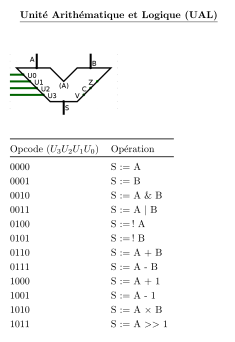
\includegraphics[width=\linewidth]{Figs/ual.pdf}\\\centering a)
   \end{minipage} \hfill
   \begin{minipage}[c]{.58\linewidth}
\includegraphics[width=\columnwidth]{Figs/ual_inner.pdf}\\\centering b)
   \end{minipage}
\caption{\label{fig:ual} a) Représentation d'une unité arithmétique et logique (UAL) disposant de $2^4 = 16$ poérations sélectionnables par l'entrée $U_3U_2U_1U_0$. Les opérandes $A$ et $B$ et la sortie $S$ sont codées ici sur 16 bits. Les signaux $N, Z, C, V$ sont les indicateurs d'états : (N: est la sortie est négative ?, Z: est ce que la sortie est nulle ? C : est ce que l'opération génère une retenue ? V: est ce que l'opération produit un dépassement de capacité. b) Une partie de l'organisation interne d'une UAL naïve avec des circuits effectuant chacune des opérations et un décodeur permettant d'en sélectionner une.}
\end{figure}

En TP, nous utiliserons des opérandes codées sur $16$ bits, donc $A$, $B$ et $S$ seront codés sur 16 bits. On représente sur la figure \ref{fig:ual}a une UAL avec $4$ bits pour sélectionner une opération (donc un total de $16$ opérations). Les signaux $N, Z, C, V$ sont les indicateurs d'états :
\begin{itemize}
\item $N$: est ce que la sortie est négative ?
\item $Z$: est ce que la sortie est nulle ?
\item $C$: est ce que l'opération génère une retenue ?
\item $V$: est ce que l'opération produit un dépassement de capacité ?
\end{itemize}
Une partie du schéma de l'UAL avec uniquement quelques opérations est représentée sur la figure \ref{fig:ual}b. Les 16 opérations sont sélectionnables par l'entrée $U$ et la table \ref{table:ual} donne le code de chacune des opérations.

\begin{table}[htbp]
\centering\begin{tabular}{c|ccc|c}
Code & Opération & & Code & Opération\\
\cline{0-1}
0000 & $S = A$ & & 1000 & $S = A+1$\\
0001 & $S = B$ & & 1001 & $S = A-1$\\
0010 & $S = A\& B$ & & 1010 & $S = A \times B$\\
0011 & $S = A|B$& &1011 & $S = A >> 1$\\
0100 & $S = \overline{A}$ & &1100 & \\
0101 & $S = \overline{B}$ & &1101 & \\
0110 & $S = A + B$ & & 1110 & \\
0111 & $S = A - B$& & 1111 & 
\end{tabular}
\caption{\label{table:ual} Exemple de code des opérations fournies par une UAL à $2^4 = 16$ opérations. Ici, seules $12$ opérations sont proposées; C'est l'UAL que nous utiliserons en TP. Pour ne pas confondre les opérations booléennes et arithmétiques sur des entiers, on note $A\&B$ le ET logique, $A|B$ le OU logique, $A+B$ l'addition. L'opération $A >> 1$ décale la représentation d'un bit sur la droite en complétant en tête par un $0$ ou un $1$ en fonction du premier bit. Sur des représentations en complément à deux, cette opération divise par deux la valeur de $A$.}
\end{table}

Il est important de retenir que l'unité arithmétique et logique n'a aucune idée du type des entrées. Les entrées $A$ et $B$ sont des paquets de bits à $0$ ou à $1$ et absolument pas des entiers, des booléens, etc... Pour le coup, il est tout à fait légitime de réaliser une opération logique sur ce que vous considérez être la représentation d'un entier. Par exemple, considérons l'opération $A\& B$ de code $U = 0010$ :
\begin{itemize}
\item avec $A = 3_{10} = 0\cdots 011$ et $B = 0\cdots 001$, on a $S = 0\cdots001$
\item avec $A= 2_{10} = 0\cdots 010$ et $B = 0\cdots 001$, on a $S= 0\cdots 000$
\end{itemize}
L'opération $A\&B$ avec $B= 0\cdots 001$ permet de tester la parité de $A$ ce qui peut être pratique si $A$ représente un entier.


%% \subsubsection{Multiplieur}



%% \begin{itemize}
%% \item table de vérité
%% \item Mentionner brièvement la combinaison de portes logiques éléments pour construire des circuits combinatoires plus compliqués, par exemple pour illustrer comment construire un additionneur, etc... vers l'UAL;
%% \item mentionner au moins le term de tableau de Karnaugh pour la synthèse
%% \item multiplex
%% \end{itemize}


\subsection{Unité arithmétique en virgule flottante}

La manipulation des représentations à virgule flottante nécessite un circuit dédié qui s'appelle Unité de calcul à virgule flottante (\emph{floating point unit}, FPU). Jusque dans les années 1990, le calcul en virgule flottante était réalisé par un processeur dédié, qui était optionnel, et indépendant du processeur ``principal'' comme par exemple les coprocesseurs Intel 8087, 80287, 80387, 80487 compagnons des processeurs Intel 8086, 80286, 80386 et 80486. De nos jours, la technologie permet d'intégrer des unités de calcul à virgule flottante directement avec le processeur principal. 

\begin{figure}[htbp]
\begin{center}
\includegraphics[width=0.5\columnwidth]{Figs/80386with387.JPG}
\end{center}
\caption{Le processeur principal Intel 80386 et son coprocesseur optionnel 80387 réalisant les opérations arithmétiques sur les représentations à virgule flottante. Source:Wikipedia.}
\end{figure}
%\todo{on peut écrire un algorithme de calcul sur les représentations flottantes avec un processeur ``principal''; quel est l'intérêt de faire un circuit dédié ??}

%%%%%%%%%%%%%%%%%%%%%%%%%%%%%%%%%%%%%%%%%%%%%%%%%%%%%%%%%%%%%%%

\pagebreak
\section{Circuits de logique séquentielle}

Dans les sections précédentes, nous avons présenté des circuits logiques dits ``combinatoires''. La sortie de ces circuits combinatoires à un instant $t$ dépends uniquement de ses entrées à ce même instant, il n'y a pas de dépendance à l'historique de la valeur des entrées\footnote{modulo les temps de propagation des signaux dans le circuit.}. Nous sommes à deux doigts de construire notre premier microprocesseur mais il nous manque encore un ingrédient. Imaginez, votre amie suzette est ornitologue, elle aimerait bien disposer d'un appareil électronique pour compter les oiseaux lors des migrations et si possible un appareil simple, par exemple avec deux boutons : un bouton pour réinitialiser le compteur et un bouton pour l'incrémenter d'une unité. Vous vous dites ``Super, je sais réaliser un additionneur, mettre une sortie à 0, c'est partie, j'écris la table de vérité''. Et là, vous êtes coincés, parce que pour une configuration d'entrée, par exemple ``bouton incrémenter pressé'', vous avez plusieurs sorties possibles : si il y avait 1 oiseau, il y en a désormais 2, mais si il y avait 2 oiseaux, il y en a désormais 3. Il vous faudrait disposer d'un moyen de représenter un \textbf{état} $n_o$ et qu'à l'appui sur le bouton vous puissiez \textbf{transiter} vers \textbf{l'état} $n_o + 1$. Dis dans l'autre sens, l'état courant dépends de l'entrée et également de l'état précédent. Cette idée est illustrée sur le schéma \ref{fig:intro_seq}. Il nous manque donc la brique permettant de mémoriser un état et c'est le sujet de cette partie.


\begin{figure}[htbp]
\centering\includegraphics[width=0.75\linewidth]{Figs/intro_seq.pdf}
\caption{\label{fig:intro_seq} Schéma de principe de n'importe quel système numérique. Etant donné un état courant et des entrées, on peut calculer des sorties et le prochain état qu'il suffit de mémoriser pour disposer d'un système dont l'influence des entrées dépends de l'état courant.}
\end{figure}



%\todo{Mentionner l'exemple de la mémoire mais peut être aussi d'un compteur}\\
%\todo{Le verrou D (D latch) peut se voir comme un mutiplexeur à 2 entrées dont l'une est sa sortie, l'autre est la donnée à mémoriser}\\

%% \subsection{Logique séquentielle synchrone et asynchrone}

%% Le verrou (\emph{latch}) est asynchrone (pas de signal d'horloge); la bascule (\emph{flip-flop}) est synchrone (avec un signal d'horloge). 

\subsection{Verrou/Bascule RS}

Le verrou RS (\emph{Reset}/\emph{Set}) possède deux entrées ($S$, $R$) et deux sorties ($Q,\bar{Q}$) comme illustré sur la figure \ref{fig:verrou_rs}. Le circuit contient des boucles de rétroaction et sa sortie est dépendante de l'historique de ses entrées comme nous allons le voir.

\begin{figure}[htbp]
\begin{center}
\tikzstyle{branch}=[fill,shape=circle,minimum size=3pt,inner sep=0pt]
\begin{tikzpicture}[label distance=2mm]

    \node[nor gate US, draw, logic gate inputs=nn] at (0,0) (Nor1) {};
    \node[nor gate US, draw, logic gate inputs=nn] at (0,-2) (Nor2) {};

    \node (S) at ($(Nor1.input 1) - (1,0)$) {$Set$};
    \node (R) at ($(Nor2.input 2) - (1,0)$) {$Reset$};
    \node (bQ) at ($(Nor1.output) + (1, 0)$) {$\bar{Q}$};
    \node (Q) at ($(Nor2.output) + (1, 0)$) {$Q$};

    \node at ($(Nor1.output) - (0.5,0)$) {$1$};
    \node at ($(Nor2.output) - (0.5,0)$) {$2$};

    \draw (S) -- (Nor1.input 1);
    \draw (Nor2.output) -- ([xshift=0.5cm]Nor2.output) -- ++(0, 0.5) -- ([xshift=-0.5cm,yshift=-0.5cm]Nor1.input 2) -- ([xshift=-0.5cm]Nor1.input 2) -- (Nor1.input 2);
    \draw (Nor1.output) -- (bQ);

    \draw (R) -- (Nor2.input 2);
    \draw (Nor1.output) -- ([xshift=0.5cm]Nor1.output) -- ++(0, -0.5) -- ([xshift=-0.5cm,yshift=+0.5cm]Nor2.input 1) -- ([xshift=-0.5cm]Nor2.input 1) -- (Nor2.input 1);
    \draw (Nor2.output) -- (Q);
\end{tikzpicture}
\end{center}
\caption{\label{fig:verrou_rs} Un verrou RS (Reset/Set) formé par deux portes NOR (les numéros dans les portes facilitent l'explication du fonctionnement du circuit) avec des connections réentrantes.}
\end{figure}

Étudions le comportement du verrou pour les entrées $(0,0)$, $(0,1)$, et $(1,0)$, on verra un peu plus loin que l'entrée $(1,1)$ conduit à un état instable et qu'on s'interdira donc cette entrée. La figure~\ref{fig:chrono_rs_1} présente l'évolution au cours du temps des entrées et des sorties du verrou. A l'instant $t_0$, l'entrée passe de $(R,S) = (0,0)$ à $(R,S) = (0,1)$. Il existe une période transitoire entre $t_0$ et $t_0 + \Delta$ avant que le circuit n'atteigne un état stable. En effet, à $t_0$, lorsque $S$ passe à $1$, seules les entrées de la première porte NOR changent. Ses entrées étant $(S, Q) = (1,0)$, la sortie passe à $\bar{Q} = 0$. Cela affecte alors à $t_0 + \Delta/2$ la deuxième porte NOR qui, ayant ses entrées à $(\bar{Q}, R) = (0,0)$ voit sa sortie passer à $Q = 1$ après un délai de $\Delta /2$. Au temps $t_0+\Delta$, les sorties du verrou sont alors à $(Q,\bar{Q}) = (1, 0)$ qui est un état stable pour le circuit. Le délai $\Delta/2$ corresponds au temps de propagation des signaux dans les portes logiques NOR et est de l'ordre de quelques dizaines à centaines de nanosecondes\footnote{Voir par exemple la notice technique de la puce 74HC02 ou CD4001}. \\

\begin{figure}[htbp]
\begin{center}
\begin{tikztimingtable}[
    timing/coldist=2pt,     % column distance
    xscale=1,yscale=1, % scale diagrams
    semithick               % set line width
]
$R$       & 2L       LLLLLL       LLLLLL       HHHHHH       LLLLLL  \\
$S$       & 2L       HHHHHH       LLLLLL       LLLLLL       LLLLLL  \\
$Q$       & 2L       LLHHHH       HHHHHH       HLLLLL       LLLLLL\\
$\bar{Q}$ & 2H N(Q1) HLLLLL N(Q2) LLLLLL N(Q3) LLHHHH N(Q4) HHHHHH \\
          & SS       SSSSSS       SSSSSS       SSSSSS       SSSSSS\\
\extracode
  %\tablerules
  %\tablegrid
  \begin{pgfonlayer}{background}
    \vertlines[help  lines]{2,4,8,14,16,20}
    \draw[thick,<->,shorten >=2pt,shorten <=2pt,>=stealth] (2, -8) -- (4,-8);
    \draw [anchor=mid] node at (3,-7) {\tiny $\Delta$};
    \draw [anchor=north] let \p1=(Q1) in node at (\x1,-9) {$t_0$};

    \draw [anchor=north] let \p1=(Q2) in node at (\x1,-9) {$t_1$};

    \draw[thick,<->,shorten >=2pt,shorten <=2pt,>=stealth] (14, -8) -- (16,-8);
    \draw [anchor=mid] node at (15,-7) {\tiny $\Delta$};
    \draw [anchor=north] let \p1=(Q3) in node at (\x1,-9) {$t_2$};

    \draw [anchor=north] let \p1=(Q4) in node at (\x1,-9) {$t_3$};
  \end{pgfonlayer}
\end{tikztimingtable}
\end{center}
\caption{\label{fig:chrono_rs_1} Chronogramme d'un verrou RS.}
\end{figure}

A l'instant $t_1$, les entrées repassent à $(R,S) = (0,0)$. Les entrées de la première porte NOR étant $(S, Q) = (0, 1)$, la sortie reste à $\bar{Q} = 0$. Pour la deuxième porte, il en est de même; ses entrées étant $(\bar{Q}, R) = (0, 0)$, sa sortie reste à $\bar{Q} = 1$. Cet état est un état de mémorisation, le verrou reste dans l'état dans lequel il était. \\

Passons maintenant, à l'instant $t_3$, les entrées à $(R,S) = (1,0)$. Seule la deuxième porte NOR voit ses entrées changer pour le moment et passer à $(\bar{Q}, R) = (0, 1)$, sa sortie passe donc à $Q = 0$. Cela a pour conséquence d'affecter la première porte; ayant les entrées $(S, Q) = (0, 0)$, sa sortie passe à $\bar{Q} = 1$. Cet état est un état stable. \\

 La table de vérité du verrou $RS$ est donnée ci-dessous~:\\
\begin{center}
\begin{tabular}{cc||ccl}
$R$ & $S$ & $Q$ & $\bar{Q}$ & Remarque\\
\hline
0 & 0 & $x$ & $\bar{x}$ & Maintien de l'état précédent\\
0 & 1 & 1 & 0 & Mise à un\\
1 & 0 & 0 & 1 & Mise à zéro\\
1 & 1 & 0 & 0 & Etat interdit 
\end{tabular}
\end{center}

\begin{framed}
\textbf{Résumé : } Un verrou RS ne s'utilise que pour les entrées $(R,S) \in \{(0,0), (0,1), (1,0)\}$.
\begin{itemize}
\item l'entrée $R=0$, $S=1$ met à 1 la sortie du verrou $Q = 1$, $\bar{Q}=0$,
\item l'entrée $R=1$, $S=0$ met à 0 la sortie du verrou $Q = 0$, $\bar{Q}=1$,
\item l'entrée $R=0$, $S=0$ laisse la sortie du verrou dans son état
\end{itemize}
\end{framed}

% 
% http://www.iitg.ernet.in/asahu/cs221/Lects/Lec13.pdf
Si les entrées $R$ et $S$ sont simultanément à un niveau haut, le système entre dans un état pour lequel les sorties $Q$ et $\bar{Q}$ ne sont pas complémentaires et est considéré comme un état interdit. En effet, le verrou peut alors entrer dans un régime instable. Si les entrées $R$ et $S$ repassent simultanément à un niveau bas $(R, S) = (0,0)$ alors que les sorties étaient également à l'état bas $(Q, \bar{Q}) = (0,0)$, dans le cas d'un circuit tout à fait symétrique, les sorties vont passer à $(1,1)$ puis $(0,0)$, ... En pratique, le circuit n'est pas parfaitement symétrique parce que les portes (et leur délais de propagation) ne sont pas tout à fait identiques et les connexions entre les sorties et les entrées non plus. Cette asymétrie conduira alors le verrou à atteindre un état stable mais en un temps arbitrairement long et il finira dans un état impossible à prédire. C'est la raison pour laquelle l'entrée $(R,S) = (1,1)$ est interdite.\\


\paragraph{Exemple : mémoriser l'appui d'un bouton:\\}

Pour illustrer l'effet mémoire d'un verrou RS, considérons deux circuits représentés sur les figures \ref{fig:ill_verrou}a et \ref{fig:ill_verrou}b. Sur la figure \ref{fig:ill_verrou}a, nous avons simplement un interrupteur qui contrôle l'allumage d'une lumière. Si on appuis sur le bouton, la lumière s'allume mais dés qu'on relâche le bouton, la lumière s'éteint. Si on modifie un peu le circuit pour placer un verrous R/S qu'on peut contrôler avec deux boutons ``allume'' et ``éteint'', on peut maintenir la lumière allumée même lorsque le bouton ``allume'' est relâché. On a donc bien mémorisé l'état ``allumé''. 

\begin{figure}[htbp]
\begin{tabular}{cc}
\begin{circuitikz}
\draw[color=black, thick]
    (0,0) to [push button,l=allume] (1.5, 0) to [lamp] (3.0, 0) to [R] (4.5, 0) to (5, 0) node[ground] {}
    (0,0) to [short,-o](0, 2) node[right]{$V^+$};
\end{circuitikz}&
\begin{circuitikz}[scale=0.9,transform shape]
\draw[color=black, thick]
    (4,0.1) node[nor gate US, draw, logic gate inputs=nn] (Nor2) {}
    (4,2.1) node[nor gate US, draw, logic gate inputs=nn] (Nor1) {}
    (0,0) to [push button,l=éteint] (2, 0) to (Nor2.input 2)
    (0,2.2) to [push button,l=allume] (2, 2.2) to (Nor1.input 1)  
    (Nor2.output) to [R] ([xshift=2.5cm]Nor2.output) to [lamp] ([xshift=3.5cm]Nor2.output) to ([xshift=4cm]Nor2.output) node[ground]{}
    (0,0) to [short,-o](0,3) node[above]{$V^+$}
    (Nor1.output) to ([xshift=.5cm]Nor1.output) node(Nor1o) {} to ([yshift=-0.5cm]Nor1o) to ([xshift=-.5cm,yshift=.5cm]Nor2.input 1) to ([xshift=-.5cm]Nor2.input 1) to (Nor2.input 1)
    (Nor2.output) to ([xshift=.5cm]Nor2.output) node(Nor2o) {} to ([yshift=0.5cm]Nor2o) to ([xshift=-.5cm,yshift=-.5cm]Nor1.input 2) to ([xshift=-.5cm]Nor1.input 2) to (Nor1.input 2)
    ([xshift=-1cm]Nor1.input 1) to [R, bipoles/length=0.5cm] ([xshift=-1cm,yshift=-1cm]Nor1.input 1) |- ([xshift=-1.5cm,yshift=-1cm]Nor1.input 1) node[ground,rotate=-90](gndpulldown) {}
    ([xshift=-1cm]Nor2.input 2) to [R, bipoles/length=0.5cm] ([xshift=-1cm,yshift=1cm]Nor2.input 2) |- (gndpulldown);
\end{circuitikz}\\
a) & b)
\end{tabular}
\caption{\label{fig:ill_verrou}a) Si le bouton est appuyé, la lumière s'allume; Si le bouton est relâché, la lumière s'éteint. b) Avec un verrou R/S, si on appuis sur le bouton ``allume'', la lumière s'allume et reste allumé même si on relâche le bouton. La lumière s'éteindra en pressant sur le bouton ``éteint''.}
\end{figure}




 L'un des inconvénients du verrou RS est que son état est tout de même très dépendant de ses entrées $R$ et $S$ puisque seul l'état $(R,S) = (0,0)$ est un état de mémoire. Il est souvent préférable d'avoir plus de contrôle sur les instants o{\`u} l'on souhaite mémoriser une donnée (fournie par R et S). On définit alors le verrou RS contrôlé (\emph{gated RS latch}) comme sur la figure~\ref{fig:gated_verrou_rs}. La seule différence avec le verrou RS est l'introduction d'un signal de contrôle qui force les entrées des portes NOR provenant de $R$ et $S$ à un niveau bas lorsque $Enable = 0$. Si $Enable=1$, ce circuit se comporte comme un verrou RS.


\begin{figure}[htbp]
\begin{center}
\tikzstyle{branch}=[fill,shape=circle,minimum size=3pt,inner sep=0pt]
\begin{tikzpicture}[label distance=2mm]

    \node[nor gate US, draw, logic gate inputs=nn] at (0,0) (Nor1) {};
    \node[nor gate US, draw, logic gate inputs=nn] at (0,-2) (Nor2) {};
    \node[and gate US, draw, logic gate inputs=nn] at ($(Nor1.input 1) - (1, 0)$) (And1) {};
    \node[and gate US, draw, logic gate inputs=nn] at ($(Nor2.input 2) - (1, 0)$) (And2) {};

    \node[anchor=east] (S) at ($(And1.input 1) - (1,0)$) {$Set$};
    \node[right] (E) at (-4,-1) {$Enable$};
    \node[anchor=east] (R) at ($(And2.input 2) - (1,0)$) {$Reset$};
    \node (bQ) at ($(Nor1.output) + (1, 0)$) {$\bar{Q}$};
    \node (Q) at ($(Nor2.output) + (1, 0)$) {$Q$};

    \node at ($(Nor1.output) - (0.5,0)$) {};
    \node at ($(Nor2.output) - (0.5,0)$) {};

    \draw (S) -- (And1.input 1);
    \draw (And1.output) -- (Nor1.input 1);
    \draw (R) -- (And2.input 2);
    \draw (And2.output) -- (Nor2.input 2);
    \draw (E) -| ($(And1.input 2)-(0.5,0)$) -- (And1.input 2);
    \draw (E) -| ($(And2.input 1)-(0.5,0)$) -- (And2.input 1);



    \draw (Nor2.output) -- ([xshift=0.5cm]Nor2.output) -- ++(0, 0.5) -- ([xshift=-0.5cm,yshift=-0.5cm]Nor1.input 2) -- ([xshift=-0.5cm]Nor1.input 2) -- (Nor1.input 2);
    \draw (Nor1.output) -- (bQ);

    \draw (Nor1.output) -- ([xshift=0.5cm]Nor1.output) -- ++(0, -0.5) -- ([xshift=-0.5cm,yshift=+0.5cm]Nor2.input 1) -- ([xshift=-0.5cm]Nor2.input 1) -- (Nor2.input 1);
    \draw (Nor2.output) -- (Q);
\end{tikzpicture}
\end{center}
\caption{\label{fig:gated_verrou_rs}Verrou RS contrôlé (\emph{gated RS latch}).}
\end{figure}

Ce verrou fonctionne sur des niveaux du signal de contrôle : lorsque le signal de contrôle \emph{enable} est à l'état haut, on retrouve un verrou RS et lorsque le signal de contrôle \emph{enable} est à l'état bas le verrou est dans un état de mémoire, peu importe ce qui se passe sur ses entrées (cf fig.\ref{fig:chrono_gated_rs_1}).

\begin{figure}[htbp]
\begin{center}
\begin{tikztimingtable}[
    timing/coldist=2pt,     % column distance
    xscale=1,yscale=1, % scale diagrams
    semithick               % set line width
]
$E$       & LH       HHHHHH       HHHLLL       LLLLLL       LLLLLL \\
$R$       & 2L       LLLLLL       LLLLLL       HHHHHH       LLLLLL  \\
$S$       & 2L       HHHHHH       LLLLLL       LLLLLL       LLLLLL  \\
$Q$       & 2L       LLHHHH       HHHHHH       HHHHHH       HHHHHH \\
$\bar{Q}$ & 2H N(Q1) HLLLLL N(Q2) LLLLLL N(Q3) LLLLLL N(Q4) LLLLLL \\
          & SS       SSSSSS       SSSSSS       SSSSSS       SSSSSS\\
\extracode
  %\tablerules
  %\tablegrid
  \begin{pgfonlayer}{background}
    \vertlines[help  lines]{2,4,8,14}
    \draw[thick,<->,shorten >=2pt,shorten <=2pt,>=stealth] (2, -10) -- (4,-10);
    \draw [anchor=mid] node at (3,-9) {\tiny $\Delta$};
    \draw [anchor=north] let \p1=(Q1) in node at (\x1,-10) {$t_0$};

    \draw [anchor=north] let \p1=(Q2) in node at (\x1,-10) {$t_1$};

    \draw [anchor=north] let \p1=(Q3) in node at (\x1,-10) {$t_2$};
  \end{pgfonlayer}
\end{tikztimingtable}
\end{center}
\caption{\label{fig:chrono_gated_rs_1} Chronogramme d'un verrou RS contrôlé.}
\end{figure}



%Le verrou RS (\emph{RS-latch}) est un circuit asynchrone: le changement de la sortie est commandé par le changement des entrées $R$ et $S$. Parfois, on souhaite contrôler 

% A voir sur les bascules D : http://www.eng.auburn.edu/~strouce/class/elec2200/elec2200-9.pdf

%\textbf{Illustration avec une mémoire 2 nor + 2 leds + 2 boutons sous logisim}

\subsection{Verrou D}

Nous sommes presque arrivé à la réalisation d'une mémoire à un bit. On souhaite mémoriser un bit, notons le $D$. Il suffit alors de considérer le verrour RS en connectant convenablement les entrées Set et Reset à $D$ comme sur la figure \ref{fig:verrou_d}

\begin{figure}[htbp]
   \begin{minipage}[c]{.7\linewidth}
\tikzstyle{branch}=[fill,shape=circle,minimum size=3pt,inner sep=0pt]
\begin{tikzpicture}[label distance=2mm]

    \node[nor gate US, draw, logic gate inputs=nn] at (0,0) (Nor1) {};
    \node[nor gate US, draw, logic gate inputs=nn] at (0,-2) (Nor2) {};
    \node[and gate US, draw, logic gate inputs=nn] at ($(Nor1.input 1) - (1, 0)$) (And1) {};
    \node[and gate US, draw, logic gate inputs=nn] at ($(Nor2.input 2) - (1, 0)$) (And2) {};
    \node[not gate US, draw] at ($(And2.input 2) - (1,0)$) (Not) {};

    \node (D) at ($(And1.input 1) - (4,0)$) {$D$};

    \node[right] (E) at (-6,-1) {$Enable$};
    \node (bQ) at ($(Nor1.output) + (1, 0)$) {$\bar{Q}$};
    \node (Q) at ($(Nor2.output) + (1, 0)$) {$Q$};

    \node at ($(Nor1.output) - (0.5,0)$) {};
    \node at ($(Nor2.output) - (0.5,0)$) {};

    \draw (D) -- (And1.input 1) node [midway,circ] (S) {};
    \draw (S) |- (Not.input);

    \draw (And1.output) -- (Nor1.input 1);
    \draw (Not.output) -- (And2.input 2);
    \draw (And2.output) -- (Nor2.input 2);
    \draw (E) -| ($(And1.input 2)-(0.5,0)$) node[midway,circ]{} -- (And1.input 2);
    \draw (E) -| ($(And2.input 1)-(0.5,0)$) -- (And2.input 1);



    \draw (Nor2.output) -- ([xshift=0.5cm]Nor2.output) -- ++(0, 0.5) -- ([xshift=-0.5cm,yshift=-0.5cm]Nor1.input 2) -- ([xshift=-0.5cm]Nor1.input 2) -- (Nor1.input 2);
    \draw (Nor1.output) -- (bQ);

    \draw (Nor1.output) -- ([xshift=0.5cm]Nor1.output) -- ++(0, -0.5) -- ([xshift=-0.5cm,yshift=+0.5cm]Nor2.input 1) -- ([xshift=-0.5cm]Nor2.input 1) -- (Nor2.input 1);
    \draw (Nor2.output) -- (Q);
\end{tikzpicture}\\\centering a)
\end{minipage}\hfill
\begin{minipage}[c]{.1\linewidth}
\includegraphics[width=\columnwidth]{Figs/verrou_D.pdf}
\\\centering b)
\end{minipage}
\caption{\label{fig:verrou_d} a) Un verrou D (\emph{Data-latch}) construit à partir d'un verrou RS en connectant les entrées Reset et Set : $Set = D, Reset = \overline{D}$. b) Représentation schématique d'un verrou D.}
\end{figure}

Ce circuit assure aussi que l'état instable du verrou $RS$ obtenu avec les entrées $R=1, S=1$ n'est jamais obtenu puisque les entrées $R$ et $S$ son câblées pour être complémentaires.

\begin{framed}
\textbf{Résumé : } Un verrou D a deux entrées $Date$ et $Enable$ et fonctionne de la manière suivante :
\begin{itemize}
\item si l'entrée $E=1$, alors $Q = D$, on dit que le verrou est transparent,
\item si l'entrée $E=0$, alors le verrou est dans un état mémoire, sa sortie ne changera pas si $D$ change et ne pourra changer que si $E$ passe à l'état haut
\end{itemize}
\end{framed}



\subsection{Systèmes logiques synchrones : horloge et fronts montants}

On précisait en introduction que le but du circuit mémoire que nous cherchons à construire est de mémoriser l'état courant d'un système, peu importe ce que représente cet état. On comprends bien que le verrou D recevra sur l'entrée D l'état mais qu'en est-il de l'entrée Enable ? On va ici considérer que la transition d'un état à un autre est rythmée par une horloge (un signal périodique en créneaux) et cela va nous conduire à construire des \emph{systèmes logiques synchrones}. Lorsque les transitions d'état sont produites par les entrées, sans être dépendantes d'un signal d'horloge, on parle de \emph{systèmes logiques asynchrones} mais nous n'en parlerons pas ici. 

Donc, pour nous, c'est une horloge qui va dicter les instants auxquels un système peut changer d'état. Un signal d'horloge est représenté sur la figure \ref{fig:clk}. Ce signal est périodique de période $T$ et de fréquence $f = 1/T$.

\begin{figure}[htbp]
\begin{center}
\begin{tikztimingtable}[
    timing/coldist=2pt,     % column distance
    xscale=1,yscale=1, % scale diagrams
    semithick               % set line width
]
$Horloge$       & 12{2C} C\\
& \\
\extracode
  %\tablerules
  %\tablegrid
  \begin{pgfonlayer}{background}
    \vertlines[help  lines]{2,6}
    \draw[thick,<->,shorten >=2pt,shorten <=2pt,>=stealth] (2, -3) -- (6,-3);
    \draw [anchor=mid] node at (4,-2) {$T$};
  \end{pgfonlayer}
\end{tikztimingtable}
\end{center}
\caption{\label{fig:clk} Un signal d'horloge est un signal en créneaux, périodique de période $T$ et de fréquence $f = 1/T$.}
\end{figure}

Si on utilise directement ce signal d'horloge comme entrée $Enable$ à un verrou D, le verrou est transparent sur le niveau haut de l'horloge comme illustré sur la figure \ref{fig:chrono_verrou_D}.

\begin{figure}[htbp]
\begin{center}
\begin{tikztimingtable}[
    timing/coldist=2pt,     % column distance
    xscale=1,yscale=2, % scale diagrams
    semithick               % set line width
]
$Horloge$ & 8L 8H 8L 8H \\
$D$       & 2L 3H 2L 2H  1L 2H 1L 1H 1L 3H  6L   2L 3H 3L \\
$Q$       & 8L 1H 1L 2H 1L 1H 1L 9H    2L 3H 3L\\
\extracode
  %\tablerules
  %\tablegrid
\end{tikztimingtable}
\end{center}
\caption{\label{fig:chrono_verrou_D} Chronogramme d'un verrou D contrôlé par une horloge. La sortie du verrou est autorisé à changer (il est transparent) tant que le signal d'horloge est au niveau haut.}
\end{figure}


Pour s'assurer qu'une seule transition ait lieu, il faut garantir que la mise à jour de la mémoire ne se fasse qu'à des instants particuliers, comme par exemple le front montant de l'horloge\footnote{on pourrait aussi considérer le front descendant de l'horloge}, lorsque ce signal passe du niveau bas $0$ au niveau haut $1$ (fig. \ref{fig:clk_fronts}). En chaînant deux verrous D, on construit ce qu'on appelle la bascule D maître escale pour laquelle on est assuré que la mise à jour de la sortie n'a lieu que sur un front d'horloge.

\begin{figure}[htbp]
\centering\includegraphics[width=0.5\linewidth]{Figs/clk_fronts.pdf}
\caption{\label{fig:clk_fronts} Le front montant d'un signal créneau est lorsque ce signal passe du niveau bas $0$ au niveau haut $1$. Le front descendant est lorsque le signal passe du niveau haut au niveau bas.}
\end{figure}

\subsection{Bascule D synchrone sur front montant : maître esclave}

En chaînant deux verrous D, on peut construire une mémoire mise à jour sur le front montant d'un signal d'horloge comme illustré sur la figure \ref{fig:flipflop_d}.

\begin{figure}[htbp]
   \begin{minipage}[c]{.7\linewidth}
\includegraphics[width=\columnwidth]{Figs/flipflop_D.pdf}\\\centering a)
\end{minipage}\hfill
\begin{minipage}[c]{.2\linewidth}
\includegraphics[width=\columnwidth]{Figs/flipflop_D_schema.pdf}
\\\centering b)
\end{minipage}
\caption{\label{fig:flipflop_d} a) Une bascule D (\emph{Data-flipflop}) construite à partir de deux verrous D respectivement appelés maître et esclave, dont la mise à jour n'est permise que sur un front montant d'horloge. b) Représentation schématique d'une bascule D. Le symbole en triangle indique un composant sensible au front montant d'horloge. Si il avait été sensible au front descendant, on aurait ajouté un petit cercle devant le triangle, à l'extérieur du composant (comme sur les portes inverseur).}
\end{figure}

Reprenons les entrées (D et Horloge) de la figure \ref{fig:chrono_verrou_D} et traçons le chronogramme des sorties des deux verrous sur la figure \ref{fig:chrono_flipflop_d}. Sur ce chronogramme, les entrées et sorties des deux verrous sont suffixés du numéro du verrou : $D_1$,$E_1$, $Q_1$ pour le premier verrou, le verrou maître et $D_2$, $E_2$ et $Q_2$ pour le second verrou, le verrou escale. Pour comprendre le fonctionnement de ce circuit, il suffit de considérer chacun des verrous l'un après l'autre en commençant par identifier quand les signaux Enable de chacun des verrous est à l'état haut et en recopiant l'entrée dans ce cas. Lorsque le signal Enable est à l'état bas, le verrou est dans l'état mémoire. Au final, si on ne se concentre que sur les entrées $D$, $Horloge$ et la sortie $Q = Q_2$, on constate que la sortie est une copie de l'entrée aux fronts montants de l'horloge, nous avons donc construit un circuit mémoire mis à jour sur les fronts montants de l'horloge (\emph{edge-triggered flip flop}).

\begin{figure}[htbp]
\begin{center}
\begin{tikztimingtable}[
    timing/coldist=2pt,     % column distance
    xscale=1,yscale=2, % scale diagrams
    semithick               % set line width
]
$Horloge$ & 8L 8H 8L 8H \\
$D=D_1$       & 2L 3H 2L 2H  1L 2H 1L 1H 1L 3H  6L   2L 3H 3L \\
$E_1$     & 8H 8L 8H 8L\\
$Q_1=D_2$     & 2L 3H 2L 1H 8H 2H 6L 8L\\
$E_2$     & 8L 8H 8L 8H\\
$Q=Q_2$       & 8L 8H 8H 8L\\
\extracode
  %\tablerules
  %\tablegrid
\end{tikztimingtable}
\end{center}
\caption{\label{fig:chrono_flipflop_d} Chronogramme d'une bascule D maître-escale sensible à un front montant d'horloge. La sortie de la bascule est la valeur de l'entrée $D$ au dernier front montant d'horloge.}
\end{figure}

Nous n'étudierons pas plus en détails le fonctionnement de la bascule D, sachez simplement qu'en pratique, le bon fonctionnement de la bascule est garantie si l'entrée est stable autour du front montant d'horloge, encadré par des temps de mise en place (\emph{setup time}) et de maintien (\emph{hold time}).

\subsection{Réalisation d'un verrou D avec un mutliplexeur}
\label{subsec:verrouD_multiplexeur}

Une autre réalisation possible d'un verrou peut se construire à partir d'un multiplexeur 2-1. Je vous rappelle qu'un multiplexeur à 2 entrées, un bit de sélection et une sortie peut être vu comme un aiguillage. Pour réaliser un verrou D avec un multiplexeur, il suffit de reboucler la sortie du multiplexeur sur la première entrée de telle sorte que si le bit de sélection vaut $0$, le circuit soit dans un état mémoire et de présenter l'entrée $D$ comme deuxième entrée du multiplexeur de telle sorte que le circuit soit transparent lorsque le bit de sélection vaut $1$. Il faudra néanmoins faire attention à utiliser la réalisation du multiplexeur sans aléas statiques. En effet, avec le multiplexeur ayant un aléa statique, si $S=1$, $D=1$ et $Q=1$, lorsque le multiplexeur est basculé dans l'état mémoire $S=1 \rightarrow S=0$, l'aléa de sortie conduit à oublier $Q=1$ et à mémoriser $Q=0$.

\subsection{Registre et mémoire RAM (Random Access Memory)}

\subsubsection{Registre à $n$ bits sur front montant}

La bascule D (maître-escale par exemple) permet de mémoriser un bit d'information et est mise à jour sur un front montant d'horloge. Pour pouvoir mémoriser un mot de plus de $n$ bits, il suffit de considérer $n$ bascules D et de construire ce qu'on appelle \textbf{un registre à n bits}, représenté sur la figure \ref{fig:registre}. Les entrées $Enable$ et $Clear$ apparaissent parfois. L'entrée $Enable$ permet d'autoriser le registre à se mettre à jour. Si l'entrée Enable est à $0$, aucune mise à jour du contenu du registre n'aura lieu. L'entrée Clear permet de remettre à $0$ le contenu du registre $Q=000\cdots$ de manière asynchrone, i.e. sans attendre de front montant d'horloge.

\begin{figure}[htbp]
   \begin{minipage}[c]{.2\linewidth}
\includegraphics[width=\columnwidth]{Figs/registre.pdf}\\\centering a)
\end{minipage}\hfill
\begin{minipage}[c]{.4\linewidth}
\includegraphics[width=\columnwidth]{Figs/registre_inner.pdf}
\\\centering b)
\end{minipage}
\caption{\label{fig:registre} a) Un registre actif sur front montant à $n$ bits. Les entrées $E$ et $Clear$ sont parfois disponibles. L'entrée $E$ autorise la mise à jour du registre et doit être au niveau haut pour que les signaux d'horloge soient opérants. L'entrée Clear permet de remettre à $0$ de manière asynchrone le contenu du registre. b) Un registre à $n$ bits sur front montant peut se construire à l'aide de $n$ bascules D sur front montant.}
\end{figure}


\subsubsection{Mémoire en lecture et écriture (RAM)}

Au même titre que combiner $n$ bascules $D$ permet de mémoriser un mot de $n$ bits, on peut aussi combiner $2^k$ registres pour mémoriser $2^k$ mots de $n$ bits comme sur la figure \ref{fig:ram}. Pour l'écriture, l'activation de l'un ou l'autre des registres se fait par l'entrée $Enable$ alimentées par la sortie d'un décodeur. Pour la lecture, le registre sélectionné par l'adresse est dirigé en sortie grâce à un multiplexeur. On dispose alors d'un contenu dit adressable. En effet l'entrée $Adr$ de $k$ bits permet de sélectionner l'un ou l'autre des $2^k$ registres soit en écriture, soit en lecture. Le choix entre l'écriture et la lecture se fait par des entrées supplémentaires Load et Store (parfois combinées en une seule).

\begin{figure}[htbp]
   \begin{minipage}[c]{.4\linewidth}
\includegraphics[width=\columnwidth]{Figs/ram.pdf}\\\centering a)
\end{minipage}\hfill
\begin{minipage}[c]{.4\linewidth}
\includegraphics[width=\columnwidth]{Figs/ram_inner.pdf}
\\\centering b)
\end{minipage}
\caption{\label{fig:ram} a) Illustration schématique d'une RAM de capacité $n 2^k$ disposant d'une entrée $D_i$ et d'une sortie $D_o$ sur $n$ bits : l'une pour le stockage l'autre pour le chargement, d'une ligne d'adresse sur $k$ bits, d'un signal d'horloge, et de signaux de contrôle pour autoriser le chargement ou le stockage de données. b) Une partie de l'organisation interne d'une RAM. Il manque sur ce schéma le circuit permettant de piloter le chargement (load) et le stockage (store) des données. }
\end{figure}

On distingue deux opérations avec les mémoires RAM : le chargement (load) et le stockage (store). Le chargement vise à placer sur le bus de données de sortie $D$, la valeur du contenu du registre adressé par l'entrée $Adr$. Le stockage vise à modifier le contenu du registre adressé par l'entrée $Adr$ avec la valeur présente sur le bus d'entrée $D$. Pour charger une valeur sur le bus de sortie il faudra :
\begin{itemize}
\item placer sur le bus d'adresse l'adresse du mot à lire
\item le mot à l'adresse $Adr$ est directement accessible sur le bus de sortie
\end{itemize}

Pour stocker une nouvelle valeur dans la mémoire, il faudra :
\begin{itemize}
\item placer sur le bus d'adresse l'adresse du mot à écrire
\item placer sur le bus de données la valeur à stocker
\item déclencher un front montant d'horloge et la nouvelle valeur sera stockée en mémoire
\end{itemize}

On parle de mémoire RAM (\emph{Random Access Memory}) puisque le temps d'accès en lecture/écriture d'un mot à une adresse donnée est indépendant de l'adresse.


%\textbf{Illustration du rôle de la bascule D : le registre à décalage}\\
%\textbf{Illustration avec le compteur par incrément : 2 bascules D avec rebouclage}\\



\vfill
\pagebreak

%%%%%%%%%%%%%%%%%%%%%%%%%%%%%%%%%%%%%%%%%%%%%%%%%%%%%%%%%%%%%%%

\section{Une première architecture interne simple d'un microprocesseur}

On dispose désormais de tout les éléments nécessaires à la réalisation d'un système de représentation et traitement d'informations numériques. La figure \ref{fig:premier_chemin_logisim} représente ce qu'on appelle un chemin de données dans lequel on reconnaît: 
\begin{itemize}
\item une unité arithmétique et logique dont les codes d'opération sont précisé dans la table~\ref{table:ual}
\item quatre registres (A, B, RADM et PC)
\item une RAM
\end{itemize}


\begin{figure}[htbp]
\includegraphics[width=\columnwidth]{Figs/premier_chemin_donnees.pdf}
\caption{\label{fig:premier_chemin_logisim} Un premier chemin de données consistué de quatre registres (A, B, RADM, PC), d'une Unité Arithmétique et Logique ainsi que de signaux de contrôles UAL, SetB, ReadB, .. tel qu'il se présente sous Logisim. La RAM est considérée comme un exemple externe au chemin de données et y est connecté par un bus d'adresse et un bus de données}
\end{figure}

Ce qu'on appelle chemin de données est l'ensemble des éléments qui permettent de traiter des informations, la RAM n'en fait pas partie en toute rigueur et doit être considéré comme un composant extérieur au chemin de données. Les données et donc la taille des bus A, B et S sont de 16 bits. Les adresses sont également codées sur 16 bits de telle sorte que la RAM contient $16 \times 2^{16}$ bits = $128$ Koctets. Ce chemin de données est celui que nous utiliserons en TP et c'est également celui que nous allons développer tout au long de ce cours pour lui ajouter quelques fonctionnalités. Les architectures actuelles utilisent de l'ordre de 8 à 32 registres internes, certains ayant des fonctions particulières et la RAM de l'ordre de quelques gigaoctets, les données et adresses étant codés sur 64 bits. 

\subsection{Registres internes : accumulateurs, registre d'adresse et compteur ordinal}

Les registres A et B vont servir à stocker les opérandes et résultats des opérations de l'UAL. Pour effectuer une opération sur des données stockées en mémoire, on s'arrangera toujours pour charger les opérandes dans les registres A et B, d'effectuer l'opération et de stocker le résultat dans un de ces deux registres et de stocker ensuite le résultat en RAM. C'est ce qu'on appelle une architecture Load/Store\footnote{qu'on oppose aux architectures registre-mémoire par exemple pour lesquelles on s'autorise à effectuer des opérations arithmétiques avec une opérande en RAM et une opérande en registre} : seules les opérations de chargement (LOAD) et de sauvegarde (STORE) accèdent à la RAM. Les opérations arithmétiques, par exemple, ne prendront jamais d'opérande directement de la RAM. C'est un choix de conception qu'on comprendra un peu plus tard.

Deux registres vont nous permettre d'accéder à la RAM : le \emph{program counter} (PC) et le \emph{registre d'adresse mémoire} (RADM). Le registre d'adresse mémoire permet de savoir à quelle adresse mémoire lire ou stocker une information. Le program counter (ou compteur ordinal) permet de savoir ou nous en sommes en RAM dans le traitement des données. 

\subsection{Séquencement du chemin de données}

Les signaux de contrôle UAL, SetB, ReadB, SetA, ... permettent d'orchestrer le chemin de données, on parle en fait de \textbf{séquencer le chemin de données}. Ce sont ces signaux de données qui vont, par exemple, permettre de faire transiter les informations entre la RAM et les registres, d'effectuer des opérations sur les valeurs en registres, de stocker les valeurs des registres en RAM, etc... Nous allons pour le moment nous concentrer sur ce qu'on va appeler un séquencement manuel, c'est à dire que nous allons considérer que nous disposons de boutons pour mettre à l'état haut ou bas ces différents signaux de contrôle et nous verrons prochainement comment automatiser cela.

\subsection{Exemple}

\label{sec:chemin_donnes_exemple}

Dans les exemples qui suivent, le séquencement du chemin de données sera illustré sur le chemin de données de la figure \ref{fig:premier_chemin}.

\begin{figure}[htbp]
\includegraphics[width=\linewidth]{Figs/premier_chemin.pdf}
\caption{\label{fig:premier_chemin} Chemin de données utilisé pour illustrer le séquencement. Pour chacun des registres, on peut visualiser son contenu. Pour plus de lisibilité, le mot de la RAM adressé par le registre RADM est souligné.}
\end{figure}

\subsubsection{Effectuer une opération sur des opérandes en RAM}

Pour mieux comprendre le fonctionnement de l'architecture, prenons un exemple. Donnons nous une RAM qui contient des données à manipuler, ici des entiers naturels, représentées dans la table~\ref{fig:ram_content1}. Cette mémoire contient deux valeurs hexadécimales : $0\times0010 = 16_{10}$ et $0\times0001 = 1_{10}$.

\begin{table}[htbp]
\centering\begin{tabular}{l|cccc}
Adresses & \multicolumn{4}{c}{Contenu}\\
\hline
0000 & 0010 & 0001 & 000A & 0000\\
0004 & 0000 & 0000 & 0000 & 0000\\
0008 & 0000 & 0000 & 0000 & 0000
\end{tabular}
\caption{\label{fig:ram_content1} Contenu de la RAM entre les adresses 0x0000 et 0x000B (la RAM étant adressable sur 16 bits, elle peut contenir $2^{16} = 65536$ mots de 16 bits, i.e. 4 chiffres hexadécimaux). }
\end{table}

Je souhaite additionner les deux opérandes aux adresses $0\times0000$ et $0\times0001$ et stocker le résultat à l'adresse $0\times000A$. Je dois donc disposer en mémoire des opérandes $0\times0000$, $0\times0001$ et aussi de l'adresse à laquelle stocker le résultat $0\times000A$. Je vous rappelle que nous respectons le principe d'architectures Load/Store, c'est à dire que les opérations arithmétiques n'ont lieu qu'entre des valeurs stockées dans les registres. Comment savoir o{\`u} nous en sommes dans le chargement des opérandes ? Grâce au registre spécial PC (\emph{program counter}, compteur ordinal) : \textbf{chaque fois qu'une opérande est ``consommée'' en mémoire, le registre PC doit être incrémenté}. Il va donc falloir :
\begin{enumerate}
\item charger la première opérande à l'adresse stockée dans PC dans un registre, par exemple le registre A, et incrémenter PC, ce qu'on notera \texttt{A:=RAM[PC]; PC := PC + 1},
\item charger la deuxième opérande à l'adresse stockée dans PC dans un registre, par exemple le registre B et incrémenter PC, ce qu'on notera \texttt{B:=RAM[PC]; PC := PC + 1},
\item additionner les opérandes et stocker le résultat dans un registre, par exemple le registre A, ce qu'on notera \texttt{A := A + B},
\item sauvegarder en mémoire, à l'adresse stockée dans la RAM à l'adresse stockée dans PC, le contenu du registre A, et incrémenter le PC, ce qu'on notera \texttt{RAM[PC] := A ; PC := PC + 1}
\end{enumerate}

Nous appellerons chacune de ces étapes des instructions. Chacune des instructions nécessitent un ensemble de sous-instruction ou micro-instruction. Prenons les les unes après les autres en considérant qu'initialement, la machine est dans l'état $RADM=0\times0000$, $A=0\times0000$, $B=0\times0000$, $PC=0\times0000$. Comme chaque micro-instruction déclenche une transition d'état de la machine, au moins un registre voit son contenu changer et comme nos registres et mémoires travaillent sur front montant d'horloge, il ne faudra pas oublier de déclencher un front montant d'horloge après avoir configuré le chemin de données (i.e. après avoir défini la valeur des signaux de contrôle). Les codes d'opération de l'UAL sont donnés dans la table~\ref{table:ual}.

Pour \textbf{charger la première opérande dans le registre A}, il faut réaliser la séquence de micro-instructions ci-dessous\footnote{les signaux de contrôle qui ne sont pas précisés sont à l'état bas $0$}, celles ci étant illustrées sur la figure~\ref{fig:premier_chemin_lda} :
\begin{enumerate}
\item diriger le PC vers RADM, donc lire le PC (ReadPC=1), transférer l'entrée A vers la sortie S pour l'UAL (UAL=0000), stocker le résultat dans RADM (SetRADM=1) \textbf{et} déclencher un front montant d'horloge
\item diriger le contenu de la mémoire vers le registre A, donc lire le contenu de la mémoire (ReadMem=1), transférer l'entrée B vers la sortie S de l'UAL (UAL=0001), stocker le résultat dans le registre A (SetA=1) \textbf{et} déclencher un front montant d'horloge
\item incrémenter le registre PC, donc lire le PC (ReadPC=1), incrémenter l'entrée A de l'UAL (UAL=1000), stocker le résultat dans le registre PC (SetPC=1) \textbf{et} déclencher un front montant d'horloge
\end{enumerate}

Après avoir exécuté cette instruction, les registres sont dans l'état suivant : $RADM=0\times0000$, $A=0\times0010$, $B=0\times000$, $PC=0\times0001$. La première instruction étant exécutée, passons à la deuxième. Pour \textbf{charger la deuxième opérande dans le registre B}, il faut réaliser la séquence de micro-instructions ci-dessous, celles ci étant illustrées sur la figure \ref{fig:premier_chemin_ldb}~:
\begin{enumerate}
\item diriger le PC vers RADM, donc lire le PC (ReadPC=1), transférer l'entrée A vers la sortie S pour l'UAL (UAL=0000), stocker le résultat dans RADM (SetRADM=1) \textbf{et} déclencher un front montant d'horloge
\item diriger le contenu de la mémoire vers le registre B, donc lire le contenu de la mémoire (ReadMem=1), transférer l'entrée B vers la sortie S de l'UAL (UAL=0001), stocker le résultat dans le registre B (SetB=1) \textbf{et} déclencher un front montant d'horloge
\item incrémenter le registre PC, donc lire le PC (ReadPC=1), incrémenter l'entrée A de l'UAL (UAL=1000), stocker le résultat dans le registre PC (SetPC=1) \textbf{et} déclencher un front montant d'horloge
\end{enumerate}

Après avoir exécuté cette instruction, les registres sont dans l'état suivant : $RADM=0\times0001$, $A=0\times0010$, $B=0\times010$, $PC=0\times0002$. Maintenant que les opérandes sont dans les registres, il faut effectuer l'opération $A:=A+B$. Pour \textbf{additionner les opérandes et stocker le résultat dans le registre A}, il faut réaliser la séquence de micro-instructions ci-dessous, celles ci étant illustrées sur la figure \ref{fig:premier_chemin_adda}~:
\begin{enumerate}
\item lire les registres A et B (ReadA=1, ReadB=1), placer en sortie de l'UAL la somme de ses entrées (UAL=0110), stocker le résultat dans le registre A (SetA=1) \textbf{et} déclencher un front montant d'horloge
\end{enumerate}


Après avoir exécuté cette instruction, les registres sont dans l'état suivant : $RADM=0\times0001$, $A=0\times0011$, $B=0\times010$, $PC=0\times0002$. Il nous reste maintenant à sauvegarder le résultat en mémoire. Pour \textbf{sauvegarder en mémoire, à l'adresse stockée dans la RAM adressée par le PC, le contenu du registre A}, il faut réaliser la séquence de micro-instructions ci-dessous, celles ci étant illustrées sur la figure \ref{fig:premier_chemin_sta}~:
\begin{enumerate}
\item diriger le PC vers RADM, donc lire le PC (ReadPC=1), transférer l'entrée A vers la sortie S pour l'UAL (UAL=0000), stocker le résultat dans RADM (SetRADM=1) \textbf{et} déclencher un front montant d'horloge
\item adresser la mémoire avec le contenu de la mémoire, donc lire la mémoire (ReadMem=1), diriger l'entrée B vers la sortie pour l'UAL (UAL=0001), stocker le résultat dans RADM (SetRADM=1) \textbf{et} déclencher un front montant d'horloge
\item stocker le contenu du registre A dans la mémoire, donc lire le registre A (ReadA=1), diriger l'entrée A vers la sortie pour l'UAL (UAL=0000), stocker le résultat en mémoire (SetMem=1) \textbf{et} déclencher un front montant d'horloge
\item incrémenter le PC donc lire le PC (ReadPC=1), incrémenter l'entrée A de l'UAL (UAL=1000), stocker le résultat dans le registre PC (SetPC=1) \textbf{et} déclencher un front montant d'horloge
\end{enumerate}


\begin{figure}[htbp]
\begin{tabular}{c}
\includegraphics[width=\linewidth]{Figs/premier_chemin_lda_1.pdf}\\
\includegraphics[width=\linewidth]{Figs/premier_chemin_lda_2.pdf}\\
\includegraphics[width=\linewidth]{Figs/premier_chemin_lda_3.pdf}
\end{tabular}
\caption{\label{fig:premier_chemin_lda} Séquence des micro-instructions permettant de charger la première opérande dans le registre A et d'incrémenter le PC.}
\end{figure}

\begin{figure}[htbp]
\begin{tabular}{c}
\includegraphics[width=\linewidth]{Figs/premier_chemin_ldb_1.pdf}\\
\includegraphics[width=\linewidth]{Figs/premier_chemin_ldb_2.pdf}\\
\includegraphics[width=\linewidth]{Figs/premier_chemin_ldb_3.pdf}
\end{tabular}
\caption{\label{fig:premier_chemin_ldb} Séquence des micro-instructions permettant de charger la deuxième opérande dans le registre B et d'incrémenter le PC.}
\end{figure}

\begin{figure}[htbp]
\begin{tabular}{c}
\includegraphics[width=\linewidth]{Figs/premier_chemin_adda.pdf}
\end{tabular}
\caption{\label{fig:premier_chemin_adda} Séquence des micro-instructions permettant d'additionner le contenu des registres A et B et de stocker le résultat dans le registre A. Notez qu'ici, il ne faut pas incrémenter le PC puisqu'aucune opérande n'a été consommée de la RAM.}
\end{figure}

\begin{figure}[htbp]
\begin{tabular}{c}
\includegraphics[width=\linewidth]{Figs/premier_chemin_sta1.pdf}\\
\includegraphics[width=\linewidth]{Figs/premier_chemin_sta2.pdf}\\
\includegraphics[width=\linewidth]{Figs/premier_chemin_sta3.pdf}\\
\includegraphics[width=\linewidth]{Figs/premier_chemin_sta4.pdf}
\end{tabular}
\caption{\label{fig:premier_chemin_sta} Séquence des micro-instructions permettant de stocker en mémoire, à l'adresse contenue dans la RAM et adressée par le PC, le contenu du registre A ainsi que d'incrémenter le PC.}
\end{figure}


\pagebreak

\subsubsection{Adressage direct des opérandes: exemple de l'incrémentation d'un compteur}

Dans l'exemple précédent, les opérandes étaient consécutives dans la mémoire. Imaginons que nous souhaitions incrémenter un compteur. On disposerait alors dans la RAM des différents incréments de notre compteur. Mais o{\`u} stocker le compteur, i.e. à quelle adresse stocker dans la RAM la valeur courant du compteur ? On va le stocker à une adresse en mémoire, par exemple, à l'adresse 0x0A. Il faut alors pouvoir charger la valeur stockée à une adresse et pour cela il nous faut introduire un nouveau mode de chargement des données en mémoire, ce qu'on appelle un \textbf{mode d'adressage}. Lorsque la valeur indexée par le registre PC en RAM est la valeur à charger (comme ce fut le cas précédemment), on parle \textbf{d'adressage immédiat}. Lorsque la valeur indexée par le registre PC en RAM est l'adresse de la valeur à charger, on parle \textbf{d'adressage direct}. Il existe d'autres modes d'adressages que nous verrons un peu plus tard.

Reprenons l'exemple précédent en changeant la RAM pour utiliser le mode d'adressage direct, comme dans la table~\ref{fig:ram_content2}. Cette fois-ci la valeur $0\times0010$ de la première opérande se trouve à l'adresse $0\times000A$. Comme précédemment, les données à utiliser sont disposées consécutivement en RAM et nous devons exécuter les instructions suivantes~:
\begin{itemize}
\item charger dans le registre A la valeur dont l'adresse est adressée par le PC en RAM (c'est de l'adressage direct) et incrémenter le PC, ce qu'on notera \texttt{A:=RAM[RAM[PC]];PC:=PC+1}
\item charger dans le registre B la valeur adressée par le PC en RAM (c'est de l'adresse immédiat), et incrémenter le PC, ce qu'on notera \texttt{B:=RAM[PC];PC:=PC+1},
\item additionner le contenu des deux registres et stocker le résultat dans le registre A, ce qu'on notera \texttt{A:=A+B},
\item sauvegarder le contenu du registre A à l'adresse adressée par le PC en RAM et incrémenter le PC , ce qu'on notera \texttt{RAM[PC]:=A;PC:=PC+1}
\end{itemize}

La seule étape qui change par rapport à l'exemple précédent est le chargement direct de l'opérande dans le registre A. Pour \textbf{charger dans le registre A la valeur dont l'adresse est adressée par le PC en RAM}, il faudra exécuter la séquence de micro-instructions suivantes~:
\begin{enumerate}
\item diriger le PC vers RADM, donc lire le PC (ReadPC=1), transférer l'entrée A vers la sortie S pour l'UAL (UAL=0000), stocker le résultat dans RADM (SetRADM=1) \textbf{et} déclencher un front montant d'horloge
\item adresser la mémoire avec le contenu de la mémoire, donc lire la mémoire (ReadMem=1), transférer l'entrée B vers la sortie S pour l'UAL (UAL=0001), stocker le résultat dans RADM (SetRADM=1) \textbf{et} déclencher un front montant d'horloge,
\item diriger le contenu de la mémoire vers le registre A, donc lire le contenu de la mémoire (ReadMem=1), transférer l'entrée B vers la sortie S de l'UAL (UAL=0001), stocker le résultat dans le registre A (SetA=1) \textbf{et} déclencher un front montant d'horloge,
\item incrémenter le registre PC, donc lire le PC (ReadPC=1), incrémenter l’entrée A de l'UAL (UAL=1000), stocker le résultat dans le registre PC (SetPC=1) \textbf{et} déclencher un front montant d’horloge.
\end{enumerate}

\begin{table}[htbp]
\centering\begin{tabular}{l|cccc}
Adresses & \multicolumn{4}{c}{Contenu}\\
\hline
0010 & 000A & 0001 & 000A & 0000\\
0004 & 0000 & 0000 & 0000 & 0000\\
0008 & 0000 & 0000 & 0010 & 0000
\end{tabular}
\caption{\label{fig:ram_content2} Contenu de la RAM entre les adresses 0x0000 et 0x000C (la RAM étant adressable sur 16 bits, elle peut contenir $2^{16} = 65536$ mots de 16 bits, i.e. 4 chiffres hexadécimaux). On souhaite incrémenter un compteur dont la valeur est mémorisée à l'adresse $0\times000A$.}
\end{table}
